%!TEX TS-program = xelatex
%!TEX encoding = UTF-8 Unicode

\documentclass{harvard-thesis}
\usepackage[toc,page]{appendix}
\usepackage{pdflscape}
\usepackage{multirow}
\usepackage{wrapfig}
\usepackage{background}

\SetBgContents{
\includegraphics{figures/header.jpg}}
\SetBgAngle{0}
\SetBgPosition{current page.north}
\SetBgOpacity{1}
\SetBgScale{1}
\SetBgColor{black}
\SetBgVshift{-1.25cm}



\renewcommand{\chapterheadstartvskip}{\vspace*{-2\baselineskip}} 

%\titleformat{\chapter}[display]{\Huge\bfseries}{\chaptername \ \thechapter}{0pt}{\vskip 20pt\raggedright}%
%\titlespacing{\chapter}{0pt}{50pt}{0pt}%


\begin{document}

% the front matter
\NoBgThispage
% some details about the thesis
\title{The DoodleBot}
\author{Anthony Evans and Rahul Victor}
\advisor{A/Prof Michael Cantoni}

% about the degree
\degree{Master of Electrical Engineering}

\degreeyear{2013}
\degreemonth{October}

% about the university
\department{Department of Electrical and Electronic Engineering}
\university{The University of Melbourne}
\universitycity{Melbourne}
\universitystate{Victoria}
\maketitle
%\copyrightpage
%\abstractpage
\tableofcontents
%\authorlist
\listoffigures
%\dedicationpage
%\acknowledgments

\onehalfspacing



% include each chapter...
%\begin{savequote}[75mm] 
%Creativity is bred from restriction.
%\qauthor{Mark Rosewater} 
%\end{savequote}

\chapter{Introduction}

%\newthought{We did not enter our task unprepared.} From the outset of our project, we understood the problems inherent in attempting to marry the wildly different expectations of our %sponsors, NHP Electrical Engineering Products and the University of Melbourne.
%One party desired beauty; a streamlined and intuitive demonstration unit. The other, a demonstration of technical prowess and the application of mathematics to reality.

%This document outlines the decisions and compromises we made in an attempt to fulfil both expectations.

%From the beginning, we realised that there would need to be a series of modules that would make up the system. There would need to be a module allowing the expression of curves that the user would like drawn, a module converting the curves into a set of movement instructions and a module that transmits those instructions to the printer. On the PLC side we would need to create a module that would receive movement instructions, a module that would interpret those instructions and a module that would cause the motor drivers to act on those instructions. A high level description of the components of the system can be seen in Fig~\ref{fig:system}.


\section{Project Overview}

\subsection{Abstract}
The DoodleBot Project was a year long undertaking completed by Rahul Victor and Anthony Evans for the  Engineering Capstone Project subject at the University of Melbourne. The produced device was a functional 2.1 axis CNC machine capable of autonomously reproducing bitmap images or photos approximated by B-splines with a pen. The device incorporates open-loop time-optimal control that attempts to complete the drawing accurately in minimum time. As an industry partner, NHP Electrical Engineering Products Pty Ltd proposed the project and provided a significant portion of the hardware for the project. This document will outline the project requirements, detail the engineered solution, justify the design and discuss performance and limitations. 

\subsection{Project Requirements}

The DoodleBot project had two key stakeholders with their own independent requirements to address and satisfy.

\subsubsection{The University of Melbourne, School of Engineering Requirements}
As part of the Bachelor of Engineering (Electrical) and Master of Engineering (Electrical) courses, students are required to complete a year long subject called the Electrical Capstone Project. Students work on completing a major engineering project designed to develop and showcase practical engineering skills and theory. The expectations of the University were outlined in the available marking criteria and subject guidelines. 

The Melbourne School of Engineering requires the following deliverables:
	\begin{itemize}
		\item A final technical report documenting the design, justification and performance of the project (this report)
		\item An oral presentation showcasing the design, justification and performance of the project
		\item A demonstration of the project at the annual Endeavour Exhibition to the general public and industry representatives
	\end{itemize}

Assessment of these is based on the following criteria:
	\begin{itemize}
		\item Demonstration of technical skill and understanding of engineering concepts
		\item Understanding relevant literature in the field
		\item Quality of design and development
		\item Quality of implementation, experimentation/testing and results
		\item Quality of presentation (for each deliverable)
	\end{itemize}
	
\subsubsection{NHP Electrical Engineering Products Pty Ltd Requirements}
The DoodleBot is an industry partnered project with NHP Electrical Engineering Products Pty Ltd (henceforth referred to as NHP). NHP's requirements for the project were agreed over several meetings and detailed in a Project Charter produced by the DoodleBot Team.

The agreed deliverables, to be handed over at the conclusion of the year, were:
	\begin{itemize}
		\item A functional device (including all hardware and software)
		\item Two promotional videos (one with a technical focus and one with a marketing focus) showcasing the features of the device
	\end{itemize}	

The specification of the product are:
	\begin{itemize}
		\item A CNC machine implemented on their specified hardware capable of 'drawing' specified programs on paper
		\item Capable of discrete 2 axis control
		\item Two state operation in third axis (on-off)
		\item Input incorporating image/photo recognition
		\item Software to be implemented on PLC and PC, with communication via a ethernet interface;
	\end{itemize}

\subsection{Project Scope}
The responsibility of the DoodleBot team was to design, implement and construct the following components:
	\begin{itemize}
		\item Control problem formulation, solution design and software implementation. Understanding of relevant control concepts
		\item Design and software implementation of image/photo input process
		\item Design and software implementation of user interface
		\item PC-PLC Network Interface design and software implementation
		\item Z-axis design and construction
		\item Wiring loom construction and assembly of components
	\end{itemize}
	
NHP's role in the project was to:
	\begin{itemize}
		\item Provide an assembled CNC frame with mechanical components for two axis movement;
		\item Provide a programmable logic controller (PLC), 2x stepper motors and 2x stepper motor PLC modules
		\item Provide adequate software and licenses for PLC programming
	\end{itemize}



\chapter{System Design}
\section{Overview}
	The DoodleBot was designed to the Project Requirements, Project Scope and Performance Indicators introduced in Chapter ~\ref{ch:intro}. An overall system architecture was designed as shown in Figure ~\ref{fig:system}. Once appropriate data types were chosen, each module of the system could be designed and tested in isolation. 
	
	This chapter will explore the engineering designs and decision that are core to DoodleBot project. The actual implementation of these designs are covered in chapter ~\ref{ch:implementation}.

\begin{figure}[h]
\centering
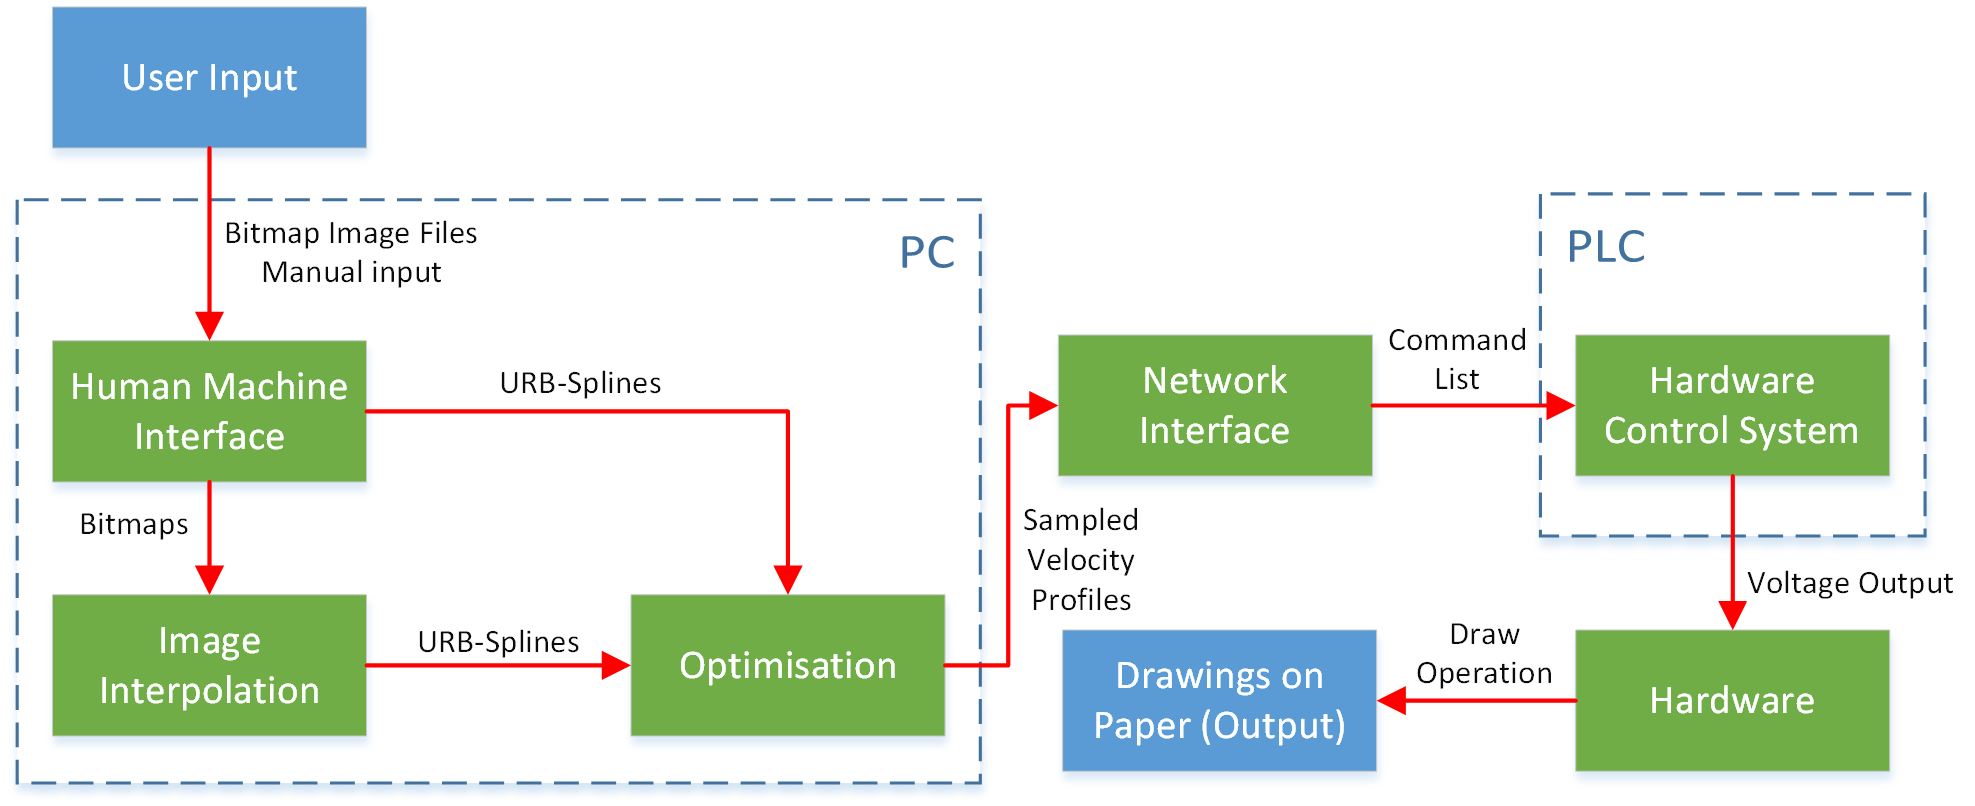
\includegraphics[width=0.9\textwidth]{figures/systemDesign/overview.png}
\caption{Modules and data flow of the DoodleBot system}
\label{fig:system}
\end{figure}

\subsection{Modules and Components}
	\subsubsection*{Input}
		The requirements stipulate a user being able to provide the machine input with photos or images. The DoodleBot was designed to accept any bitmap format (including compressed formats such as JPEG or PNG), but was optimized for simple images such as logos and photos of simple photographs with simple, distinct objects (such as buildings or hand drawn sketches on paper/whiteboards).
		
		In addition to this, the DoodleBot provides the added functionality of allowing the user to define URB-Splines directly through the Human-Machine Interface Interface.
		
	\subsubsection*{Output}
		The required output is a representation of the input to be drawn onto paper in a single colour via the DoodleBot mechanical hardware.
		
	\subsubsection*{Human-Machine Interface (HMI)} 
		The Human-Machine Interface (HMI) is the only way for a user to interact with the DoodleBot system and features an simple interface that includes the capability to provide both methods of input - selecting bitmap image files stored on the computer and a way to intuitively construct URB-Splines. Another important feature would be a way to control various parameters used in the optimisation process for testing purposes.
		
	\subsubsection*{Quadratic URB-Splines}
		The quadratic Uniform Rational Basis Spline (URBS) was chosen as the data type into the optimisation section. It is a versatile way of representing various curves with very little data and is defined by mathematical equations that are convenient for the optimisation calculations. See Section ~\ref{sec:design-urbs}.
		
	\subsubsection*{Image to Spline Interpolation}
		The Image to spline interpolation module takes the bitmap image input to the DoodleBot and generates a representation of the input in terms of Quadratic URB-Splines for use by the optimisation module. This module is what generates the reference image that the hardware tries to ultimately draw onto the paper (ie, the output). See Section ~\ref{sec:design-interpolation}.
		
	\subsubsection*{Optimisation}
		Two of the performance indicators identified in Chapter ~\ref{ch:intro} were related to how fast and how accurate the device can draw the image onto the output medium. The Optimisation module takes the input URB-Splines and generates velocity profiles (for use in the Hardware Control module) that are time optimal for given hardware constraints. See Section ~\ref{sec:design-optimisation}.

	\subsubsection*{Network Interface}
		One of the requirements of the project was to construct a network interface between the Programmable Logic Controller and the PC using an Ethernet connection. The network interface allows the sampled velocity profiles to be sent from the PC to PLC and includes software on both devices. 

	\subsubsection*{Hardware Control System}
		The Hardware Control System takes sampled velocity profiles for each axis and drives the two motors to match these profiles. The Hardware Control System also controls the two-state control of the Z-axis (draw functionality). Project requirements stipulated this module to be implemented on the Programmable Logic Controller. See Section ~\ref{sec:design-control}.

%URBS
\section{Uniform Rational Basis Splines}
\subsection{Introduction to URBS}

\subsection{Design Rationale}

The decision to use URBS as a method of restricting and structuring the input curve type was made for several reasons. 

Firstly the structure that a spline based representation gives to the input data gives natural compression for that data, as compared to storing the location of each individual point upon the desired curve. This effect is easily seen when compared to an array based method of storing curve data for single given line. A number of integers on the order of 20 can store the same amount of data as thousands of bits. However, this effectiveness goes down when approximating a high density of curves per unit of area. In our application, the average density of curve was to be very low. Thus, an URBS curve fit well for data compression. 

This paradigm also allows for easy storage and manipulation of input curves by the GUI program. It also decouples the size and form of the curve from any functions that interact with it, as the curves all have a standard form and all data only represents objects that are of interest. This means that computation interactions were easier to design and were intrinsically flexible to alterations in the makeup of the URBS curves. With an array based method altering something as simple as the relative size of a data set to be printed would create problems and require patches to most of the functions that make up the pathway from data to printing commands.

The restriction of the curves to splines of the 3rd order ensures that the parametrised curve has the property of being twice differentiable;
\begin{align*}
\textbf{q}(s) \in \mathbb{C}^2
\end{align*}
Where $\textbf{q}(s)$ represents the position of each axis with respect to a point along the curve.
If this were not the case, the path velocity could not be be guaranteed to be continuous. The plant would then require infinite acceleration at those discontinuities in order to travel the path at any speed. Thus a 3rd order URBS curve can be guaranteed to be traversable by a system with finite force input without any halt to its movement. Each curve can be swept in a single motion in a continuous manner. This results in fast traversal of the path, allowing the mechanism to complete its tasks in a short amount of time.

Finally, the parametrisation of the curve $\textbf{q}(s)$, allows us to easily retrieve the path velocity $\textbf{q}'(s) = \frac{dq(s)}{ds}$ and path acceleration $\textbf{q}''(s) =  \frac{d^2q(s)}{ds^2}$ unambiguously at any point on the curve. This is vital in calculating the forces required for a path traversal at any given $\dot{s}(t)$. The requirements of the path can thus be analysed with a view to perfect traversal accuracy. In comparison, an array based method would have a path velocity which would need to be estimated based on discrete position data. The method used to extract the path velocities would be inherently inaccurate.

The URBS curve has a few limitations in implementation, particularly with complexities involved the creation of a spline to represent a target image. However when a movement command is in a spline format it guarantees properties which result in easy application of optimisation calculations and the overall accuracy of command output.
\subsection{URBS Analysis}
Given their benefits, 3rd order URBS were used as the curve data structure for the DoodleBot. 

The general weighting structure of an URBS is the same for each and every curve, given the uniformity of their knots. This means that we can easily calculate the basis functions for an URBS given only the number of control points. Thus an URBS curve is completely defined by the number and location of its control points.

A knot vector is a set of numbers which define the locations of all of the knots that a curve contains. An URBS contains only evenly spaced knots. The knot vector defines the knot spans of a curve. Over each span, only three control points will have non-zero weighting. At the end of each span, one control point's weighting goes to zero and is substituted by another control point, whose weighting begins from zero also. The numeric values of the knots within the vector are unimportant; the curve parametrising variable $s$ starts from the first knot and ends at the last and all knots are evenly spaced. We have arbitrarily defined the knots such that all lie between zero and one.

The knot vector defines weighting coefficients for each of the control points. The values of these weights quadratically shifts across the domain of $s \in [0, 1]$. This brings consecutive control points into prominence evenly as the path parameter is traversed. Each point on the curve consists of a linear combination of the control points that are non-zero for the knot span. This is demonstrated in the following equation
\begin{align*}
q_i(s) = w_i\textbf{N}_i^2 + w_{i-1}\textbf{N}_{i-1}^2 + w_{i-2}\textbf{N}_{i-2}^2
\end{align*} 
Where $q_i(s)$ is a point on the path with $s$ inside the $i$th knot span and $N_i^2$ is the $i$th control point.

When the $s$ parameter passes a knot value such as $s = 0.5$ in Fig~\ref{fig:urbsDemo}, it changes the knot span it is within. This signifies that the lowest indexed control point no longer has influence over the position of the path and the control point corresponding to the index of the new knot span will begin to rise in weighting.

In this way each point on the curve is defined by a linear combination of three control points and each control point has weighted influence over a similar sized domain on $s$. The weightings for each control point can be determined given the knot vector.

The knot vector can be obtained by applying the following algorithm, where $N$ is defined as the number of control points.
\begin{align*}
K_3 &= \left[0, 0, 0, 1, 1, 1\right]\\  
K_4 &= \left[0, 0, 0, \frac{1}{2}, 1, 1, 1\right]\\  
K_5 &= \left[0, 0, 0, \frac{1}{3}, \frac{2}{3}, 1, 1, 1\right]\\
K_N &= \left[0, 0, 0, \frac{1}{N-2},\frac{2}{N-2} \cdots ,\frac{N-2}{N-2}, 1, 1\right]\\  
\textit{subject to}\\
N &\geq 3\\
N &\in \mathbb{Z}
\end{align*}

Note that there are three repeated knots at the beginning and end of a curve. The knot span of these points each has a width of zero, meaning that the curve does not exist inside these spans. These knots make sure that the curve terminates at the location of the first and last control point. They also ensure that the weighting functions have defined values throughout the recursive calculations.

The knot vector can be calculated when one is given the number of control points of a curve. Given the knot vector we can use the recursive definition of URBS basis functions to calculate the the control point weightings for any given $s \in [0, 1]$
\begin{align*}
W_{i}^d(s) &=   \frac{s - K_i}{K_{i+d} - K_i}W_{i}^{d-1}(s)  +  \frac{K_{i + d + 1} - s}{K_{i + d + 1} - K_{i+1}}W_{i+1}^{d-1}(s)\\
W_{i}^0(s) &= \begin{cases}
   1 & \text{if } K_i \leq s < K_{i+1} \\
   0 & \text{otherwise}
  \end{cases}
\end{align*}
Where $K_i$ is the knot at index $i$ and $d$ is the dimension of the URBS curve.

For the cases where the multiplying fractions result in $\frac{0}{0}$, we take the result to be $0$.

When the URBS curve is of dimension 2 the line equation for $q_i(s) = q(s)\bigm|_{K_i \leq s < K_{i+1}}$ results in the following definition \cite{website:nurbsExplain};
\begin{align*}
q_i(s) = \textbf{N}_i^2W_{i}^{2}(s) + \textbf{N}_{i-1}^2W_{i-1}^{2}(s) + \textbf{N}_{i-2}^2W_{i-2}^{2}(s)
\end{align*}
Where $\textbf{N}_i^2 = \begin{bmatrix}
x_i\\y_i
\end{bmatrix}$ is the $i$th control point and $W_{i}^{2}(s)$ is the second order basis weighting corresponding to that control point. 
For details of the derivation and closed form of $W_{i}^{2}(s)$, please see Appendix A.

Given the piecewise form of the line, one can easily take the derivative of $\textbf{q}(s)$ with respect to $s$ and obtain the path velocity $\frac{d\textbf{q}(s)}{ds} = \textbf{q}'(s)$ and path acceleration $\frac{d^2\textbf{q}(s)}{ds^2} = \textbf{q}''(s)$. This results in the derivative of $W_{i}^{2}(s)$ with respect to $s$ alongside the same control points and knot indexes, calculating the result in a manner exactly the same as for the position.

%Control System
\section{Control System and Optimisation}
\subsection{Open Loop Control System}
	The DoodleBot uses two stepper motors in open loop to control the position and movement of the drawing head (open loop justification in Section~\ref{sec:control-stepper}). The input to the system is the frequency of voltage pulses and the output is the velocity of the drawing head. 
	
	Both the input and output operate in 'step' units (see Section~\ref*{sec:implementation-mechanical} for more detail on what this unit is in the real system).
	
	For this system to operate as required, there are constraints on the maximum acceleration the system can run at.
	
	\subsubsection{Stepper Motors and Open Loop Justification}
		\label{sec:control-stepper}
		\begin{figure}[h]
			\centering
			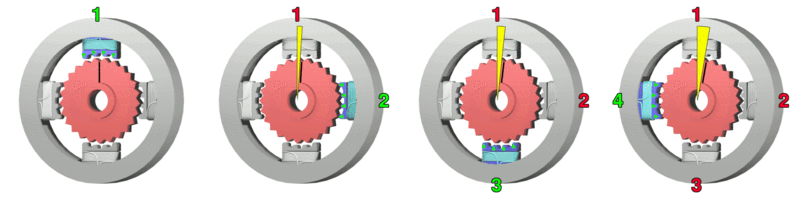
\includegraphics[width=0.8\textwidth]{figures/optimisation/steppermotor}
			\caption{Operation of a simplified stepper motor over four steps}
			\label{fig:stepper}
		\end{figure}
			
		Stepper Motors are brushless DC motors and are used as the primary drivers for X and Y movement in the DoodleBot. Where a standard DC motor creates an output torque proportional to input current, a stepper motor rotates at a speed that matches the frequency of input voltage steps.
		
		As shown in Figure~\ref{fig:stepper}, stepper motors consist of several electromagnets arranged in a equally spaced pattern around a gear-shaped rotor. Each electromagnet is shaped to have its own teeth that can align with the rotor's teeth. 
		
		When the stepper motor driver receives a single voltage step, it provides a constant current to the first electromagnet, creating magnetic force that rotates the rotor a small amount (a single step) such that the teeth on the rotor gear align with the teeth on the magnet. Damping in the mechanical system prevent oscillations about this point. As long as the input voltage pulse is maintained, this electromagnet will remain active.
		
		When the first electromagnet is aligned with the rotor teeth, the second electromagnet will be out of alignment. When a second input voltage pulse is received, the stepper motor driver will activate the second electromagnet, causing the rotor to make another rotation step such that it is now in alignment with the second electromagnet. This process continues sequentially across numerous electromagnets around the rotor.
		
		The important thing to note is that the speed of rotation is proportional to the frequency in which the input voltage pulses are received. As long as the magnetic force provided by the electromagnet is enough for the rotor to make the required step within the time the electromagnet is active, the mechanical load on the rotor does not effect the average speed at all. A lighter load may allow the individual step to be quicker, but as the second step will not be made until the next input pulse is received, the differences between a heavy and light load are negligible.
		
		This behaviour means that within certain torque constraints, the stepper motor is a robust and predictable device that we can run in open loop. Since the loads on the system do not vary significantly between possible states (the gravitational force is always the same orientation for all states and mass is constant) the torque constraint can be approximated by an acceleration constraint.
\subsection{Purpose}
In Section ~\ref{fig:control}, an open-loop control system was designed that would accurately be able to reproduce certain velocity profiles within certain acceleration constraints - a design requirement that would limit the time it takes the DoodleBot to draw. The Performance Indicators defined in Chapter ~\ref{ch:intro} specified drawing time as an attribute to minimize.

The purpose of the time optimisation module is to make maximal use of the available power of the stepper motors without exceeding their acceleration constraints, minimizing the time taken to draw while allowing the open loop control system to operate as required.

\subsection{Path Velocity Optimisation}
A machine that follows prescribed paths has an inherent trade-off between obeying the physical restrictions of the device and following a path at the fastest possible speed. There is a wealth of information surrounding the topic of the optimisation of such physical systems, seen in \cite{Bardine10},  \cite{Chen07}, \cite{Choi01}, \cite{Tseng09}, \cite{Schutter09} and \cite{Yeh99}. Each study was relevant to the optimisation problem present in the DoodleBot system, but used differing strategies and overcame different limitations to achieve a trajectory that minimised some particular cost. The method most relevant to the project, and the one that was chosen to implement was \cite{Schutter09}. A comparison of the different optimisation strategies is instructive and can be seen in Appendix B.

The dynamics of the drawing head can be viewed as a double integrator system. With limits on $\ddot{\textbf{q}}(t)  = \begin{bmatrix}
\frac{d^2x(t)}{dt^2}\\
\frac{d^2y(t)}{dt^2}
\end{bmatrix}= \begin{bmatrix}
\ddot{x}(t)\\
\ddot{y}(t)
\end{bmatrix}$, an equality can be constructed that will impose limits on the trajectory of each of the two axes in following the path. The specifics of the path and the speed of its traversal can be separated via the path parametrisation $s$.
\begin{align*}
\textbf{q}(s) &= \sum^N_{i=1}\textbf{N}^2_iW_{i,2}(s) = \begin{bmatrix}
x(s)\\
y(s)
\end{bmatrix}\\
\textbf{q}(t) &= \textbf{q}\left(s(t)\right)\\
\end{align*}
Here, the mechanism of the separation of concerns is apparent. A function $s(t)$ is constructed which represents the progress along the path as a function of time. It was previously stated in Section ~\ref{sec:design-urbs} that:
\begin{align*}
s(t_0) &= 0\\
s(t_f) &= 1\\
s(t) &\in [0,1] 
\end{align*}
Which means that the plant starts at the beginning of the path $s = 0$ at $t_0$ and completes its movement at the end of the path $s = 1$ at $t_f$. The derivatives of $\textbf{q}(t)$ can be found with respect to time in terms of the properties of the path $\textbf{q}(s)$ and the time derivatives of a traversal trajectory $s(t)$ as follows;
\begin{align*}
\dot{\textbf{q}}(t) &= \frac{d\textbf{q}}{ds} \frac{ds}{dt}\\
\ddot{\textbf{q}}(t) &= \frac{d}{dt}\left(\frac{d\textbf{q}}{ds}\right)\frac{ds}{dt} +  \frac{d\textbf{q}}{ds}\frac{d^2s}{dt^2}\\
 &= \frac{d^2\textbf{q}}{ds^2}\left(\frac{ds}{dt}\right)^2 +  \frac{d\textbf{q}}{ds}\frac{d^2s}{dt^2}\\
 \ddot{\textbf{q}}(t) &= \textbf{q}''(t)\dot{s}^2(t) + \textbf{q}'(t)\ddot{s}(t)
\end{align*}
Where $\textbf{q}''(t) = \frac{d^2\textbf{q}(s)}{ds^2}$, $\textbf{q}'(t) = \frac{d\textbf{q}(s)}{ds}$, $\dot{s}(t) = \frac{ds}{dt}$ and $\ddot{s}(t) = \frac{d^2s}{dt^2}$.

The problem can be simply stated as choosing $\dot{s}(t)$ such that 
\begin{align*}
\ddot{\textbf{q}}_{min} \leq \ddot{\textbf{q}}(t) \leq \ddot{\textbf{q}}_{max}
\end{align*} 
This can be stated intuitively as attempting to minimise the time taken for the completion of a specific path without exceeding the torque limitations of a plant.

The problem faced in minimising the time taken is that there are points known as switching points in the trajectory of $s(t)$ which occur when the path velocity $\dot{s}(t)$ needs to decrease in order to be able to clear a section of the curve without breaking the constraints. In order to minimise the time taken to traverse the curve, there are switching points in the trajectory of $s(t)$ when a difficult section of curve is completed. At these points the path velocity should be increasing as much as possible within the bounds of the constraints. This result of maximum acceleration and deceleration is known as 'Bang Bang' control and is typical in the result of time-optimal calculations. This result is intuitive when one considers that the actuators are performing at their limits at all stages of the curve.
 
To find the solution that minimises the completion time these key acceleration and deceleration switching points need to be identified. The identification of these points gives the positions where the system should begin to accelerate and decelerate along the path.
In order to find these switching points to obtain the minimum time of traversal a few options are available.

One could attempt to determine the limiting axis at each point on the curve and then determine the optimal points for switching between accelerating and decelerating the path velocity via iterative shooting methods to meet the imposed limitations. This result will give the global optimum for the minimum time of path traversal, given the constraints. A drawback of this problem is that it is a difficult problem to solve for the general case.

A simpler and more robust option is to break the path into discrete segments, calculate the maximum $\textbf{q}'(s)$ and $\textbf{q}''(s)$ for each segment and accelerate along the path such that these maximum values are satisfied at the commencement of and during each of these discrete divisions along the path. This method is a discrete approximation of the continuous method outlined above. As such the answer that results is an approximation of the global optimum. This arises as limits are generated for the sections of the path, which might be confined to a small area. These limiting areas are artificially spread out with the discretisation of the path. Thus the problem that is solved is not an accurate representation of the true problem. However we are able to generate constraints on the system that match the true constraints, which will not be exceeded. The ensuing calculation will minimise the time of completion for the approximated system. Thus the approximated solution will approach the global solution as the granularity and hence accuracy of the discrete approximation increases.

Once all of the switching points are identified, the optimal path trajectory $s^*(t)$ can be easily calculated, from which desired velocities and positions along $x^*(t)$ and $y^*(t)$ can also be calculated.

Formally, the problem to be solved is expressed by;
\begin{align*}
\min_{T, \; s(\cdot)} \;& \int_0^T1dt\\
\text{subject to} \quad \ddot{\textbf{q}}(t) &= \textbf{q}'(t)\ddot{s}(t) + \textbf{q}''(t)\dot{s}^2(t)\\
s(0) &= 0\\
s(T) &= 1\\
\dot{s}(0) &= 0\\
\dot{s}(T) &= 0\\
\dot{s}(t) &\geq 0\\
\ddot{\textbf{q}}_{min} &\leq \ddot{\textbf{q}}(t) \leq \ddot{\textbf{q}}_{max}\\
\text{for } t &\in [0,T]\\
\end{align*}
\subsubsection{Pontryagin's Maximum Principle}

We set about attempting to solve the optimal control problem utilising Pontryagin's Maximum Principle. Despite our best efforts, we found the problem to be intractable to solve in the general case.
The major confounding factor we had in finding a continuous and completely optimal solution to our problem lies in the construction of a representation for the interaction of the path constraints on the separate axes.
One can construct a Hamiltonian

\subsection{Linear and Convex Optimisation Approach}
The method used to solve the problem involved breaking the curve down into a discrete number of sections and solving the continuous problem in a piecewise manner, which allows for the restrictions to be more easily considered.

The problem is now to apply a numerical solving method in order to find the approximated optimum. Using the technique outlined in \cite{Schutter09}, the problem was reformulated such that the non-linear constraint $\ddot{\textbf{q}}(t) = \textbf{q}'(t)\ddot{s}(t) + \textbf{q}''(t)\dot{s}^2(t)$ becomes linear for the solution variables, whilst the cost function remains convex. Enforcing linearity in the solution variables allows for the solution to be found by efficient solvers, as well as ensuring that a solver will not be able to get caught in a local minima.
The key to this linearisation is representing the non-linear portion of the constraint $\dot{s}^2(t)$ with the solution variable $b(s)$ as so;
\begin{align*}
a(s) = \ddot{s}(s)\\
b(s) = \dot{s}^2(s)
\end{align*}
Such that the non-linear constraint becomes
\begin{align*}
\ddot{\textbf{q}}(s) = \textbf{q}'(s)a(s) + \textbf{q}''(s)b(s)
\end{align*}
Note that the time dependence of the path parametrisation is neglected. This is because the cost function is reformulated with a change of variables such that its dependence on $t$ is replaced by a dependence on $s$. Thus the solution that minimises the cost function will minimise the time taken implicitly without direct reference to time as shown here;

\begin{align*}
J(T) &= \int_0^T1\;dt\\
J(s(\cdot)) &= \int_{s(0)}^{s(T)} \frac{1}{\dot{s}}ds\\
	&= \int_0^1\frac{1}{\dot{s}}ds
\end{align*}

The cost function is trying to minimise the inverse of $\dot{s}(t)$, which is the equivalent of attempting to maximise the path velocity. Given the goal is to solve for $b(s) = \dot{s}^2(s)$, the cost can be formulated in terms of our solution variable;
\begin{align*}
J(s(\cdot)) = \int_0^1\frac{1}{\sqrt{b(s)}}ds
\end{align*}

The change of variables gives us a cost that remains convex and is in terms of one of the solution variables.
\subsection{Discretisation of Path}

The results of this alteration to our problem are far reaching. Firstly, it can be seen that our problem is now linear in its constraints. This results in our viable solution space taking up a contiguous range, meaning that for the solver no isolated solutions are unreachable.
Secondly, the cost integral that integrates over the trajectory $s$ is convex in the solution variable $b(s)$, so that a solver will always be able to determine the correct direction to move the state such that it converges to the local optimum.
With the combination of these two properties, it can be seen that a solver can be employed to correctly solve for the optimal trajectory $\dot{s}^*(s)$, through the solution of $b^*(s)$

In order to form a discrete problem that a computer can iterate over and solve, the path is discretised and the trajectory is solved over each path segment. As the control input, $a(s)$ is given as being piecewise constant for each discrete segment of $s$. Thus, as it is finite and constrained by the system constraints. $\sqrt{b(s)}$ is piecewise linear and continuous, meaning $b(s)$ is piecewise non-linear and continuous. 
\subsubsection{SeDuMi}

The discretised optimisation problem is formulated into a second order cone solver, SeDuMi so as to be solved with numerical efficiency. For each segment, the bounds on $b(s)$ and $a(s)$ are defined with respect to the acceleration constraints. The calculation of the maximum $\textbf{q}''(s)$ and $\textbf{q}'(s)$ for each discretised path section gives the constraints. The starting and finishing values of $b(s)$ are anchored to zero. Finally, two solution variables are introduced in order to enable the efficiency of a second order cone program. $c(s)$ is introduced as $\sqrt{b(s)}$ and $d(s)$ is introduced as the increment of the cost integral.
The entire solving functionality was automated and wrapped in a function that could solve the optimal trajectory for a curve  given simply an URBS representation and the torque constraints.

\subsection{Results}
Here, the process that a curve undergoes from initialisation to the generation of the final velocity profile will be demonstrated, drawing upon the theoretical underpinnings of the previous sections.
Firstly, a curve is obtained through manual manipulation of control points or by extraction from image features. The curve that will be taken through the optimisation process can be seen in Figure \ref{fig:example}. The curve has seven control points and has a complex shape that will incur several changes in the limiting axis and hence contain several switching points, demonstrating the ability of our optimisation process to drive the machine to the limits of its physical limitations.

\begin{figure}[htbp]  
\centering
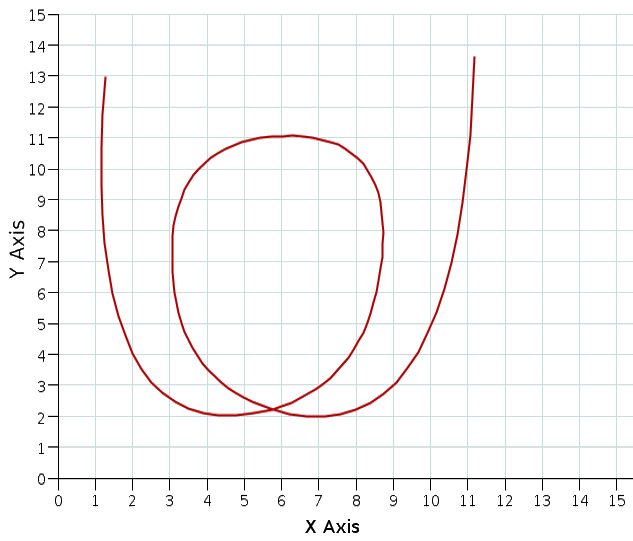
\includegraphics[width=0.7\textwidth]{figures/optimisation/exampleSpline.png}
\caption[Optimisation example curve]{ This spline has 7 control points and 10 knots. This example will be used to demonstrate the properties of URBS curves and the optimisation process.
\label{fig:example}}
\end{figure}

The spline is decomposed into its X and Y axis coordinates, giving the positions that each axis should achieve at each point on the curve. The result of these parametrisations can be seen in Fig.\ref{fig:xy_s}. Bundled onto the same graph with these curves is the simulated final product of the optimisation and transmission process. It can be seen that the black curve representing the final theoretical output at this level of zoom has an error that is nearly imperceptible. The deviation that is discernible from the correct path is not an artefact of the optimisation process. The velocity profile sampling which is required to pass the movement information across to the plant discretises the velocity information, which causes accumulating integration error.\footnote{Further work would include an interpolation scheme based on the sampling rate that would adjust these profiles such that the machine would be back on the curve after each sampling period. This implementation is not trivial as the adjustments to the velocity discretisation may cause the acceleration constraints to become exceeded.} However it can be seen in Fig.\ref{fig:xy_s} that the final effect is slight. These effects are also reset at the culmination of each curve. Thus the introduced error was considered to be within allowable bounds for our purposes.

\begin{figure}[htbp]
\centering
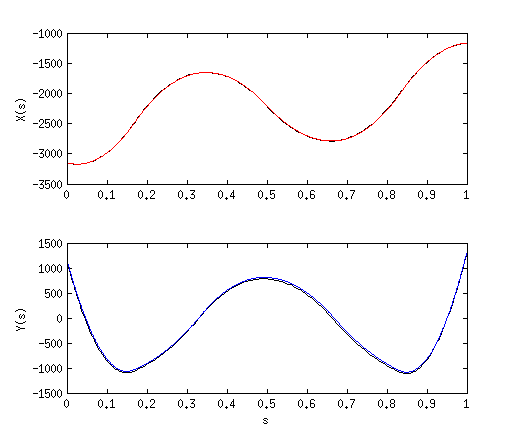
\includegraphics[width=0.7\textwidth]{figures/optimisation/xy_s.png}
\caption[Indexed curve position and theoretical final path]{
The X axis (TOP) and Y axis (BOTTOM) displaying the correct trajectory in colour and the approximated path that will be followed in black, given a velocity profile that is sampled at 25Hz.
\label{fig:xy_s}}
\end{figure} 

The discretisation aspect discussed in previous sections mentioned that the problem required a discrete approximation of the derivatives of the given path. The URBS curve used can easily have the parametrised curve derivatives ($\textbf{q}'(t)$ and $\textbf{q}''(t)$) extracted at each discretisation point for the SeDuMi solver. The curves for the first and second derivatives of the axis position with respect to the parametrisation variable for the path in the example spline seen in Fig~\ref{fig:example} can be seen in Fig~\ref{fig:xy_dds_ds}. These values are extracted by taking the derivative of the quadratic URBS weighting equations with respect to the parametrisation variable $s$.
Unsurprisingly the first derivative is piecewise linear and continuous. Thus, it is quite easy to find the maximum value for a given discrete section and thus encode the discrete approximation with the requisite path parameters.
The second derivative is piecewise linear. Finding something that would be considered a limiting value over a discrete path section is a little troublesome here, as the value can jump to differing discrete states. This issue can actually cause the discrete approximation of the constraints to be invalid for low sampling values, as will be discussed later.

\begin{figure}[htbp]
\centering
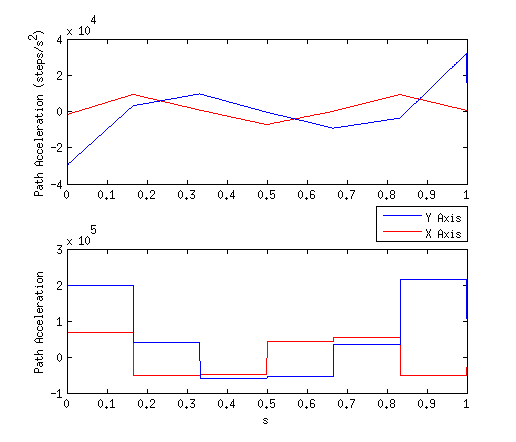
\includegraphics[width=0.7\textwidth]{figures/optimisation/xy_dds_ds.png}
\caption[Parametrised curve derivatives]{
The first (TOP) and second (BOTTOM) derivatives of the parametrised curve position for the example curve. Note the discrete jumps in level for the second derivative and the corresponding changes in gradient for the first derivative.
\label{fig:xy_dds_ds}}
\end{figure}

Given that there is a discretised problem with appropriate constraints, the solver SeDuMi can compute the discrete $\dot{s}^*(s)$, which is the approximated time optimal trajectory. The trajectory which was arrived at for the given example curve can be seen in Fig.~\ref{fig:sdot_st}.
The final calculation step in order to achieve the desired $s^*(t)$ requires that we compute the resulting time $t$ for each $s(s)$ via the inverse relation
\begin{align*}
t(s) &= \int_0^s\frac{1}{\dot{s}^*(s)}du\\ 
\end{align*}

\begin{figure}[htbp]
\centering
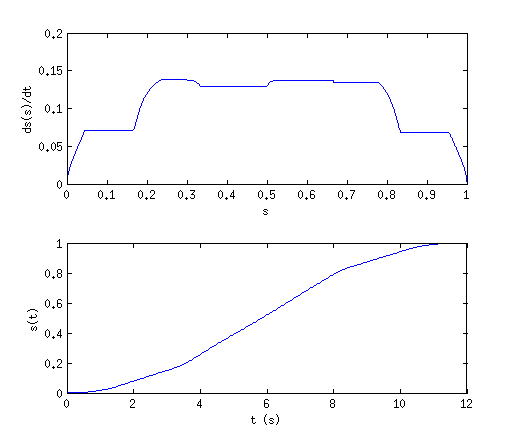
\includegraphics[width=0.7\textwidth]{figures/optimisation/sdot_st.png}
\caption[$\dot{s}^*(s)$ and $s^*(t)$]{
The optimal curve velocity (TOP) and the retrieved path trajectory (BOTTOM) for the example curve.
\label{fig:sdot_st}}
\end{figure}

Since $\dot{s}^*(s)$ is defined in a piecewise non-linear fashion due to its direct relation to the piecewise linear trajectory $b(s)$, a mapping between $t$ and $s$ for arbitrary $t$ can be obtained via the algorithm outlined in Appendix B. The output $s(t)$ can be seen in Fig.~\ref{fig:sdot_st}. Though the solution can be solved for a piecewise closed form, the required output data type of the Optimisation module is a sampled velocity profile, so an algorithm that solves for a given discrete sampling rate $k\Delta T$ is used. This allows for an a desired velocity sampling frequency to be specified and subsequently calculated using sampled values of $s(k\Delta T)$ to generate the sampled velocity profile via 
\begin{align*}
\frac{d\textbf{q}\left(k \Delta T\right)}{dt} &= \frac{\textbf{q}\left(s(k\Delta T)\right)}{ds}\frac{ds(k\Delta T)}{dt}
\end{align*}
Hence, the process has generated the optimal axis velocity curves that can be sent to the unit in order to faithfully follow a URBS curve with a time optimal trajectory.
An output of the time optimal trajectory $\dot{\textbf{q}}(k\Delta T)$ and $\ddot{\textbf{q}}(k\Delta T)$ can be seen in Fig.~\ref{fig:bangbang}.

\begin{figure}[htbp]
\centering
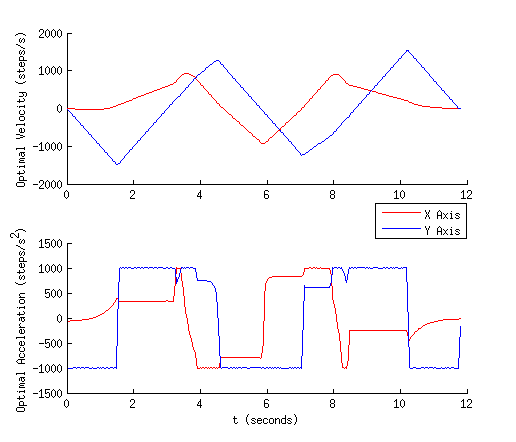
\includegraphics[width=0.7\textwidth]{figures/optimisation/bangbang_xy_ddt_dt.png}
\caption[$\dot{\textbf{q}}^*(t)$ and $\ddot{\textbf{q}}^*(t)$]{
The time optimal axis velocity (TOP) and the time optimal axis acceleration (BOTTOM) for the example curve.
\label{fig:bangbang}}
\end{figure}


\section{Image Interpolation}
\chapter{Implementation}
\label{ch:implementation}
\section{Overview}
	The overall system was designed in Chapter ~\ref{ch:design}. This chapter will explore the hardware and software used to implement the theoretical design to create a functional product.

%CNC machine
\section{Mechanical}
\label{sec:implementation-mechanical}

	\subsection{Frame}
	
		\subsubsection{Motors}
	
		\subsubsection{Limit Switches}
	
	\subsection{Drawing Head - Z-axis}
	
	
\section{Electrical and Wiring}

	\begin{figure}[h]
		\centering
		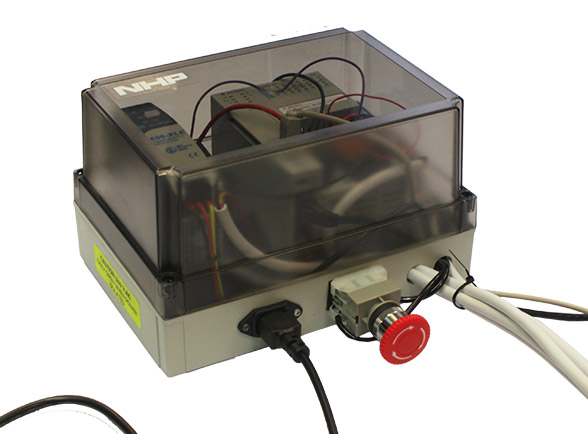
\includegraphics[width=0.5\textwidth]{figures/cncMachine/control.jpg}
		\caption{DoodleBot Control Enclosure}
		\label{fig:control}
	\end{figure}
	
	The wiring diagram in Figure ~\ref{fig:WiringDiagram} shows electrical layout of the system. The DoodleBot has two major groups of components - the electronics and control components sit in the DoodleBot Control Enclosure (Figure ~\ref{fig:control}) and the electromechanical components are mounted to the DoodleBot CNC Frame (Figure ~\ref{fig:implementation-mechanical}).

	
\begin{landscape}
		\vspace*{\fill}
		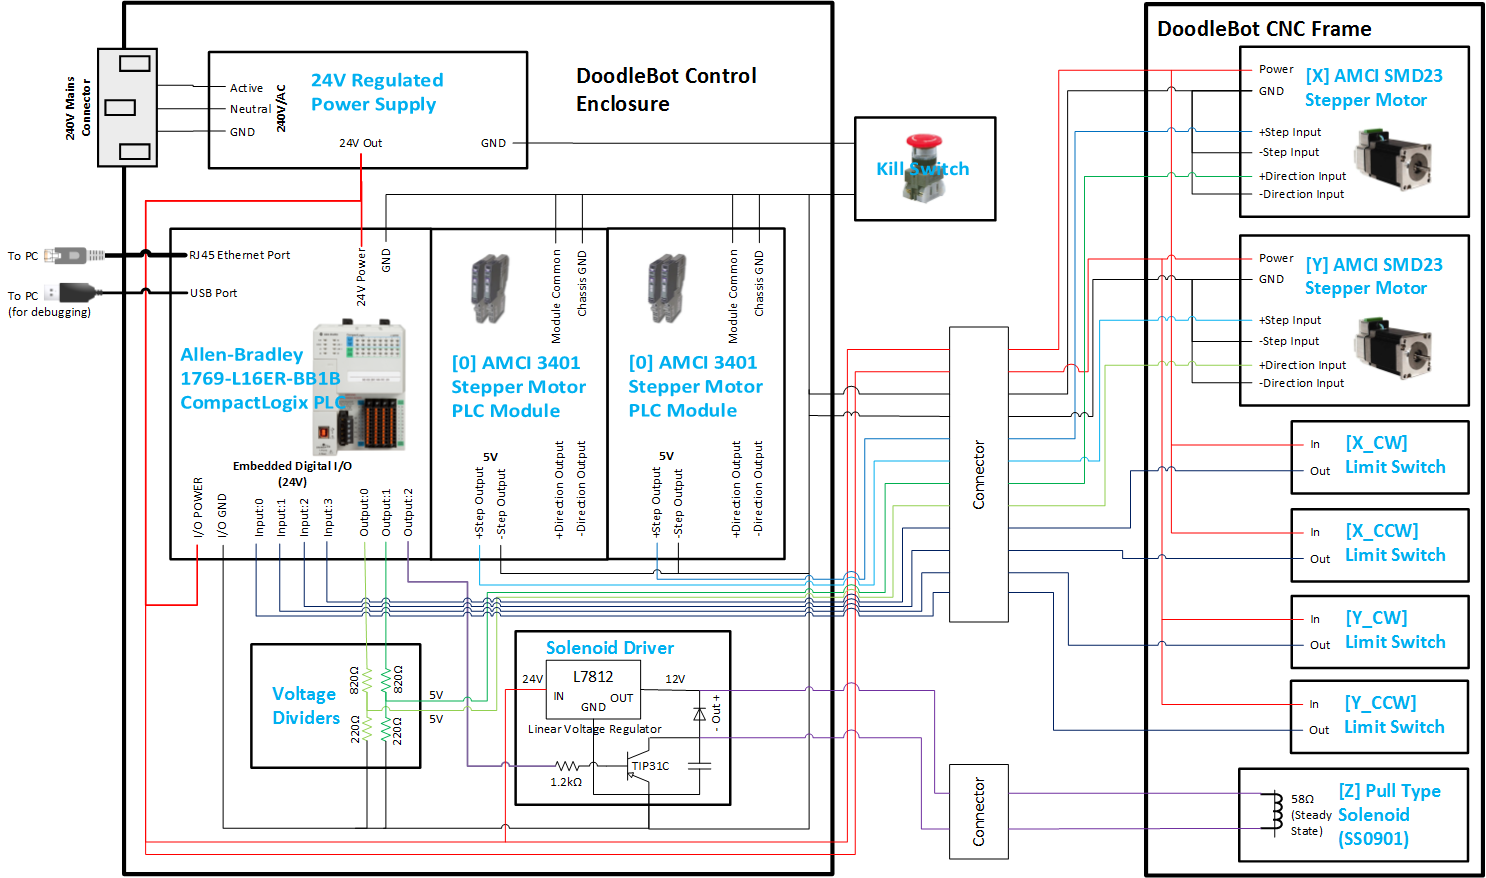
\includegraphics[width=\hsize]{figures/cncMachine/wiring}
		\captionof{figure}{Wiring Diagram}
		\label{fig:WiringDiagram}
		\vspace*{\fill}
\end{landscape}


	\subsection{Connectors and Loom}
	
	The DoodleBot team constructed a 14-wire loom to transmit power and signals between the Control Enclosure and the CNC Frame. Figure ~\ref{fig:loom} shows the plastic connector pin outs and Table ~\ref{table:loom} lists the details of each wire/pin in the loom.
		\begin{figure}[h]
			\centering
			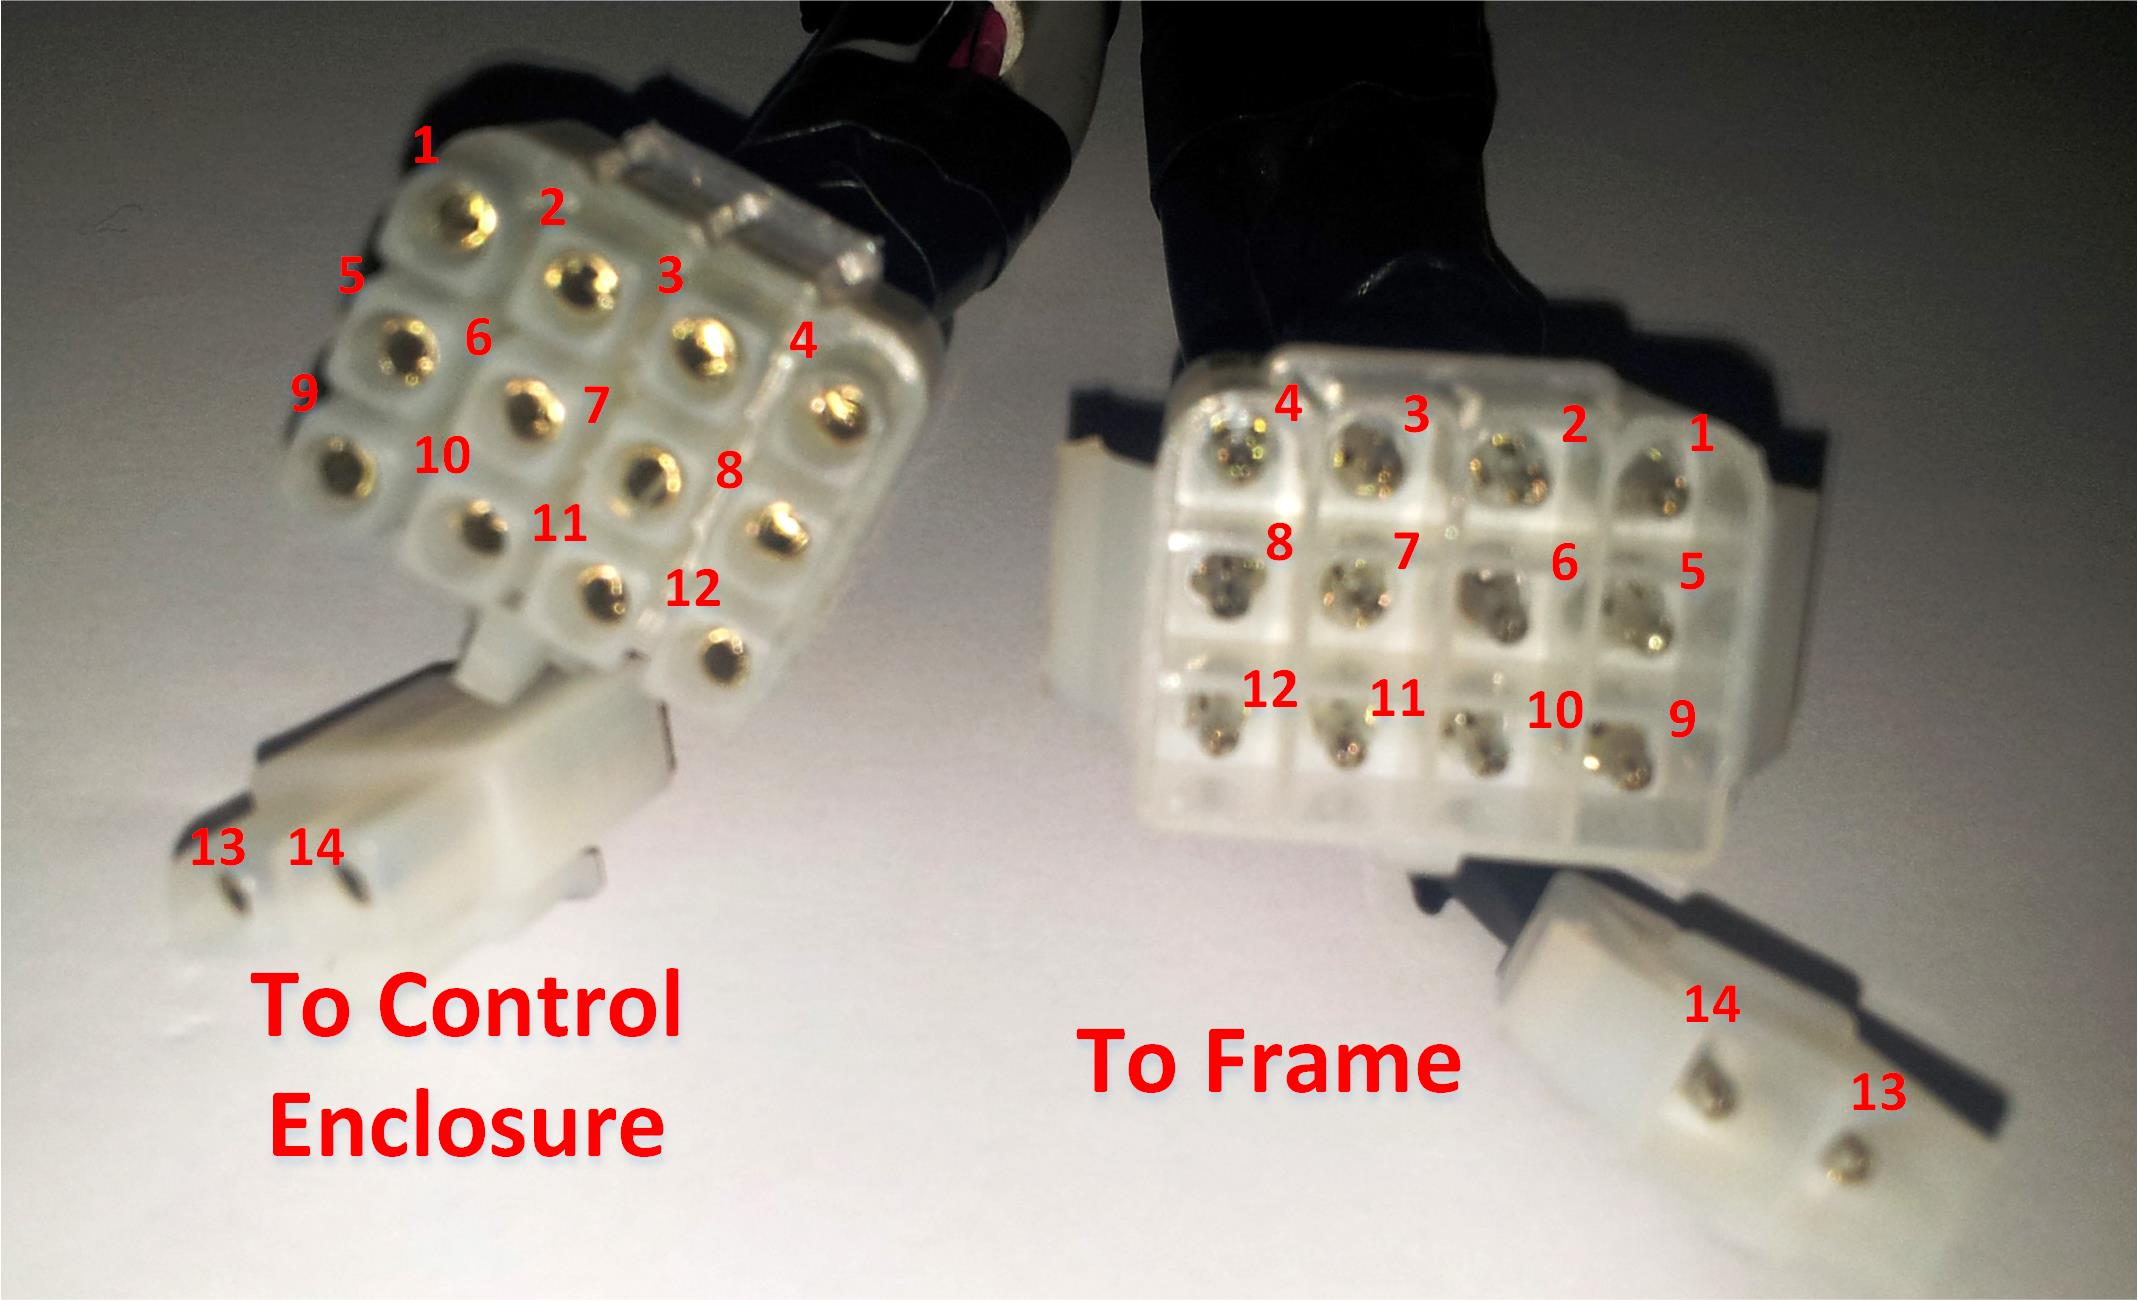
\includegraphics[width=0.5\textwidth]{figures/cncMachine/loom.jpg}
			\caption{Wiring Loom Connector Pin out}
			\label{fig:loom}
		\end{figure}
		
		\begin{table}[h]
			\centering
			\begin{tabular}{|c|c|c|l|l|}
				\hline
				\emph{Pin} & \emph{Wire Colour} & Voltage & \emph{Control Enclosure Side} & \emph{CNC Frame Side} \\ \hline
				1 & Red & 24V & Power & \parbox[t]{6cm}{SMD23 +PWR [X] \\ Limit Switch [X\_CW],[X\_CCW]} \\ \hline
				2 & Red/Yellow & 5.1V & PLC DC Output 0 & SMD23 +Direction [X]\\ \hline
				3 & Red & 5V &  3401 Step Output [0] & SMD23 +Step [X]\\ \hline
				4 & Black & 0V & GND & SMD23 -PWR, -Direction, -Step [X] \\ \hline
				5 & Red/Yellow & 24V & Power & \parbox[t]{6cm}{SMD23 +PWR [Y]\\ Limit Switch [Y\_CW],[Y\_CCW]}\\ \hline
				6 & Black/Yellow & 5.1V & PLC DC Output 1 & Stepper Motor Direction [Y]\\ \hline
				7 & Black & 5V &  3401 Step Output [1] & SMD23 +Step [Y]\\ \hline
				8 & Black/Yellow & 0V & GND & SMD23 -PWR, -Direction, -Step [Y] \\ \hline
				9 & Black & 24V & PLC DC Input 0 & Limit Switch [X\_CW]\\ \hline
				10 & Black/Yellow & 24V & PLC DC Input 1 & Limit Switch [X\_CCW]\\ \hline
				11 & Red & 24V & PLC DC Input 2 & Limit Switch [Y\_CW]\\ \hline
				12 & Red/Yellow & 24V & PLC DC Input 3 & Limit Switch [Y\_CCW]\\ \hline
				13 & Red/Yellow & 12V & +Solenoid Driver Output & +Solenoid [Z]\\ \hline
				14 & Black & 0V & -Solenoid Driver Output & -Solenoid[Z]\\ \hline
			\end{tabular}
			\caption{Wiring loom and connector specifications}
			\label{table:loom}
		\end{table}
	\subsection{Voltage Dividers}
		The direction signals for the stepper motors are produced from the PLC on pins $embedded.DCout.0$ and $embedded.DCout.1$ at $24V$. The AMCI SMD23 only accepts a differential input of $5V$.
		
		Since the AMCI SMD23 direction input is a digital signal (ie, high impedance input), we can use a simple voltage divider circuit to produce the correct voltage. 
		
		The PLC embedded output can produce a maximum of $500mA$ per pin. One important thing to consider however, is it requires a \emph{minimum} of $1mA$ from each pin while in the on-state to operate properly. 
		
		Choosing resistors of $820\Omega$ and $220\Omega$ in the voltage dividers give a $5.08V$ output and draw $2.3mA$, satisfying the minimum current condition. 
	\subsection{Solenoid Driver}
		A Jaycar SS0901 pull-type solenoid is used to control the drawing head operation.
		
		The solenoid is designed to operate at $12V$, has a resistance of $58\Omega$ and an unknown inductance. In steady state operation it draws $207mA$ and consumes $6W$. The solenoid can be modelled as an R-L circuit: an off-on transition will begin with current draw of $0mA$ and transiently approach $207mA$. In an on-off transition, there will be a large spike of negative current which gradually reduces to zero as the inductor component discharges.
		
		The PLC embedded output can produce a maximum of $500mA$ per pin. One important thing to consider however, is it requires a \emph{minimum} of $1mA$ from each pin while in the on-state to operate properly. 
		
		Due to the transient behaviour of the solenoid, a simple voltage divider cannot be used. Instead an STMicroelectronics L7812 Linear Voltage Regulator in TO220 packaging is used to perform the $24V-12V$ DC-DC conversion. $6W$ of power is lost as heat in the L7812 during the on-state and so a heatsink is used and the housing for the circuit is vented.
		
		Due to the minimum current requirement of the PLC output, a TIP31C bipolar junction transistor (BJT) is used as the solenoid switch. A field effect transistor (FET) would not work since it would not draw enough current to allow the PLC output to operate properly.
		
		To meet the $207mA$ required by the solenoid, there is a minimum current requirement through the base of the BJT. The TIP31C datasheet shows that tested with a collector-emitter current of 1A, the minimum DC current gain is 25. So at least $8.28mA$ is required through the base. A more conservative value of $20mA$ is chosen by placing a $1.2k\Omega$ resistor in between the PLC output and BJT base.
		
		To allow the inductor to discharge quickly (and without damaging other components), a flyback switching power diode is put across the Solenoid Driver Output in reverse orientation. In the on-off transition, the inductor discharge current (flowing in the reverse direction of normal current flow) will have an alternate path to follow and energy will dissipate as heat in the solenoid and diode. This protects other electronic components as well allowing the solenoid to be more responsive in dropping its load.
		
	\subsection{Kill Switch}
		The DoodleBot features a kill switch (emergency stop switch) mounted to Control Enclosure that disconnects the power supply's GND output from all the powered components. 
		
		It should be noted that the power supply itself continues to operate and energy storage components in the rest of the circuit (eg, inductors and capacitors) will retain their charge.



\section{Hardware Control Software}

This section gives an overview to the design of the hardware control system, implemented on a Programmable Logic Controller. For more detailed information on how this module is implemented on the PLC, please see Appendix ~\ref{ch:PLC-flowcharts}.

\subsection{Introduction to Programmable Logic Controllers}
	Programmable logic controllers (PLCs) are computers designed for control and automation of mechanical hardware. They are designed to be robust and used in harsh environments. They have hardened I/O designed to be less susceptible to electrical noise, power surges, shorts etc. The physical units are very durable and designed for large temperature ranges and to be impact/vibration resistant.
	
	PLCs differ from micro controller boards as they come with a rudimentary operating system. The operating system is hardened against things such as memory faults and forces code to be valid before being run. They also feature control over program task management and can guarantee tasks being run at deterministic time intervals. The operating systems are usually designed with networking capability including directly sharing variable data, or even storing variable data remotely. Another major advantage is the ability to be able to be reprogrammed over a variety of interfaces (USB, Ethernet, etc) while live and in operation (important in machinery that cannot be taken off-line or stopped). They are also more deterministic than general purpose PCs, providing more reliable and predictable code execution.
	
	Each PLC can only be programmed by manufacturer propriety software via standard programming methods defined in the IEC 61131-3 standard. These include three visual languages: ladder diagrams, functional block diagrams and sequential functional charts, and two text based languages: structured text and instruction lists.
	
\subsection{PLC Hardware}
	\subsubsection{Allen-Bradley 5370-CompactLogix 1769-L16ER-BB1B}
		The PLC unit provided by NHP for the DoodleBot project is the Allen-Bradley 5370-CompactLogix 1769-L16ER-BB1B. Allen-Bradley is a well known, industrial-quality brand within Rockwell Automation's automation family of products. The PLC features 16 24V-sinking embedded DC input ports and 16 24V-sourcing embedded DC output ports, has 2 embedded Ethernet ports and a USB slave port. It has the capability of up to 16 expansion modules. The unit is programmed by the RSLogix5000 software.
	\subsubsection{AMCI 3401 Stepper Motor Module}
		The DoodleBot uses 2 AMCI 3401 stepper motor modules added to the PLC to control the AMCI SMD23 stepper motors fitted to the DoodleBot CNC Frame. The AMCI 3401 modules monitors some reserved variables in the PLC memory which are used to control the module through specified commands. There are a large variety of move types and configuration commands that can be used. Based on these, the modules control the rotation of the stepper motor modules via producing a step signal output and direction signal output that can be read by the SMD23 stepper motor integrated drivers.
		
		For more detailed information on the AMCI 3401 moduels and how they are used by the DoodleBot system, see Appendix ~\ref{sec:PLC-flowcharts-amci}.
\subsection{PLC Program Architecture}
		Figure ~\ref{fig:PLCarchitecture} shows the overall architecture and input/output flow of the PLC module. The programmable logic controller has four programs that run in parallel and perform different tasks. Each task has its own program scope memory and can be viewed as wholly independent state machines. They interface with each through globally scoped variables and share important data as well. All programs are implemented in ladder diagrams. 
		
		The programs are:	
		\begin{description}
			\item[Governor] \hfill \\
				The Governor state machine sets the overall state of the DoodleBot controller by interfacing with Communications and motorControl.
			\item[Communications] \hfill \\
				The Communications state machine is in charge of managing the UDP socket interface, all network communications and the populating of the command list.
			\item[motorControl] \hfill \\
				The motorControl state machine's job is to control all the electromechanical components on the DoodleBot Frame - primarily the stepper motors and drawing head. It also uses communicates with the checkLimitSwitch program.
			\item[checkLimitSwitch] \hfill \\
				The checkLimitSwitch program periodically monitors the limit switch input and triggers an emergency stop if the switches are triggered. It runs every 10ms.
		\end{description}
		
		The DoodleBot also makes use of 4 of the embedded DC input ports to read the input from the Limit Switches and 3 of the embedded DC output ports to (2 to control stepper motor direction and the third to control the solenoid). The embedded Ethernet socket interface is also used for the PC-PLC network interface. USB is also used to program/debug the PLC. 
		
		For more information on why the direction input of the stepper motors are controlled by the PLC and not using the Direction Signal Output on the stepper motor modules, please see Section ~\ref{sec:stepperdirectionmanagement}.
		
				See Table ~\ref{table:globalvariables} for further detail on the structures of the global variables and Table ~\ref{table:progaminterfaces} for more detail on the possible states of the program interfaces, both in Appendix ~\ref{ch:PLC-flowcharts}.
		

\begin{landscape}
		\vspace*{\fill}
		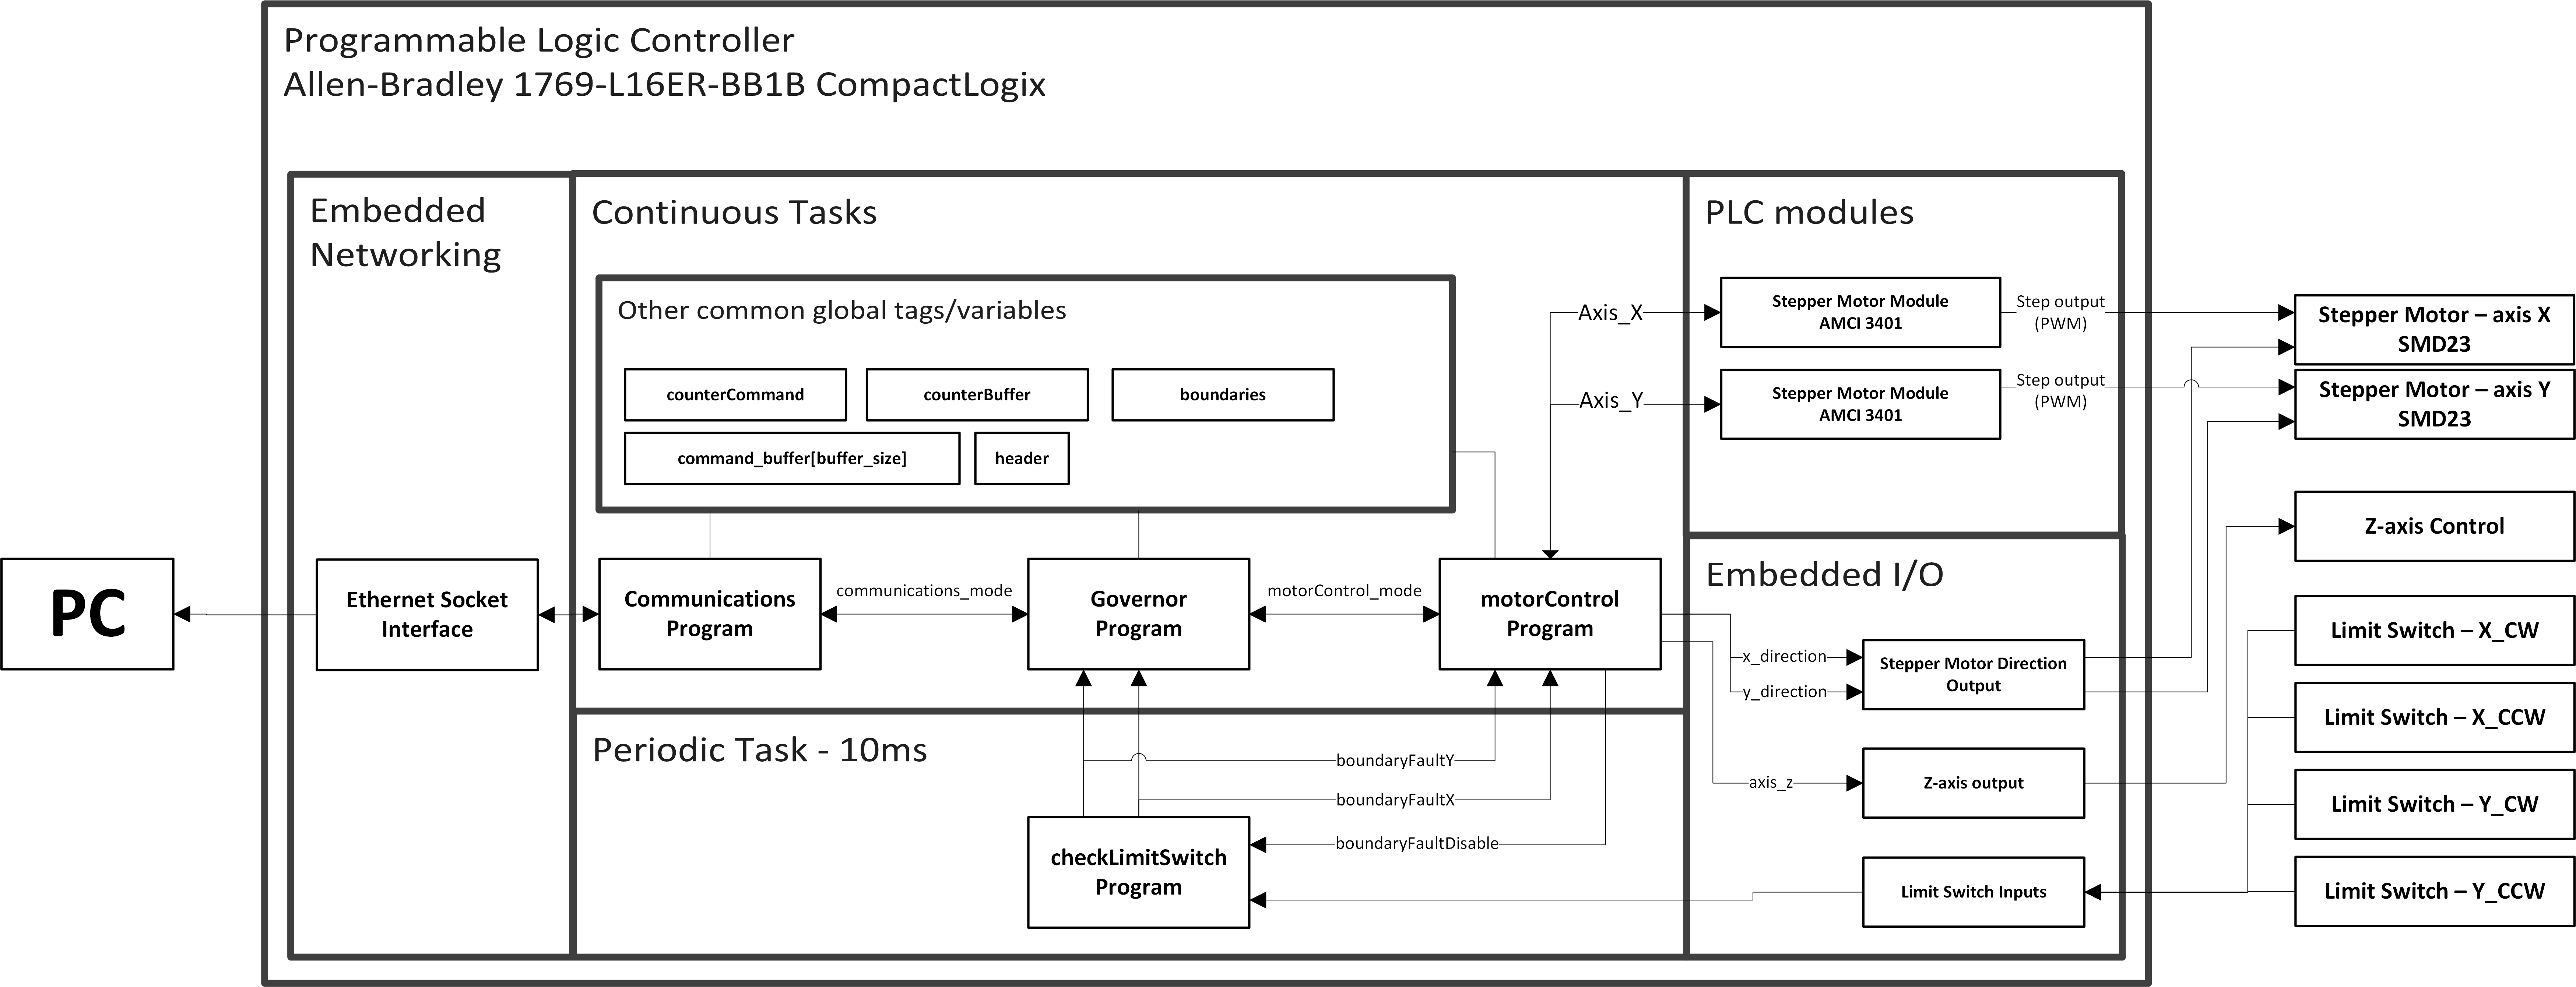
\includegraphics[width=\hsize]{figures/cncMachine/PLC_architecture}
		\captionof{figure}[PLC Architecture and I/O]{The program and I/O architecture of the PLC. Arrows represent data flow, and when labelled, are global scope variables.}
		\label{fig:PLCarchitecture}
		\vspace*{\fill}
\end{landscape}



	\subsection{Governor}
	
		\begin{figure}[h]
			\centering
			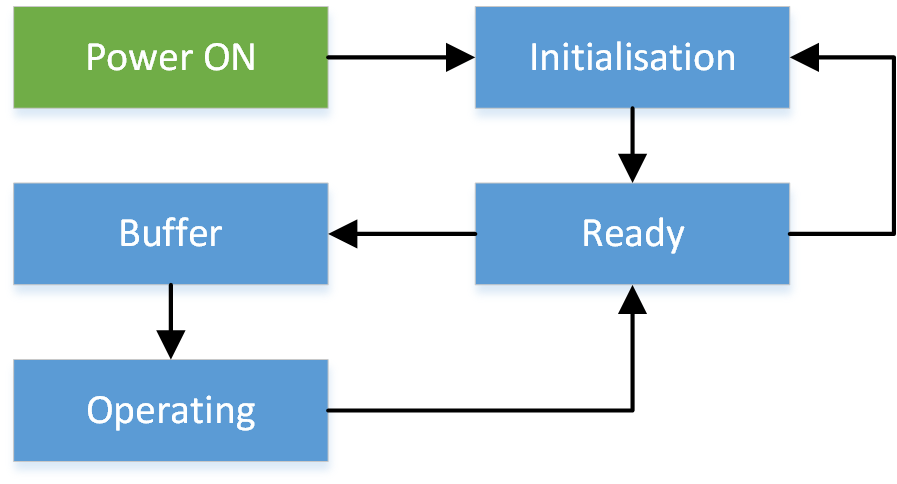
\includegraphics[width=0.5\textwidth]{figures/cncMachine/governor_simple.png}
			\caption{Governor States}
			\label{fig:governor-states}
		\end{figure}
		
		The Governor, shown in Figure ~\ref{fig:governor-states}, is a state machine that control the operation of the other programs in the DoodleBot system. The states are:
		
		\begin{description}
			\item[Power ON] DoodleBot waits for the user to press one of the Y limit switches to state A to start initialization.
			\item[Initialisation] The DoodleBot checks the boundaries and centres itself on a 'home' position. After this is complete it progresses to state B.
			\item[ready] The DoodleBot starts sending the 'ready' packet periodically to the PC, while waiting for a header to arrive. If a valid header arrives, it transitions to state C. If one of the Y limit switches are pressed, it returns to state A to run through the initialization routine once more.
			\item[Buffer] The DoodleBot begins requesting commands from the PC, filling the commandBuffer. When either the commandBuffer is full or all commands have been received, it progresses to state D.
			\item[Operating] The DoodleBot begins executing the commands in the commandBuffer. If there are still commands to received, it will continue to buffer when slots are freed up after being executed. After all commands have been processed the system returns to state B, ready for another header.
		\end{description}
		
		Please see Figure ~\ref{fig:PLC-flowcharts-governor} in Appendix ~\ref{ch:PLC-flowcharts} for more detailed information on how the Governor operates.

\subsection{Communications}
	
			\begin{figure}[h]
				\centering
				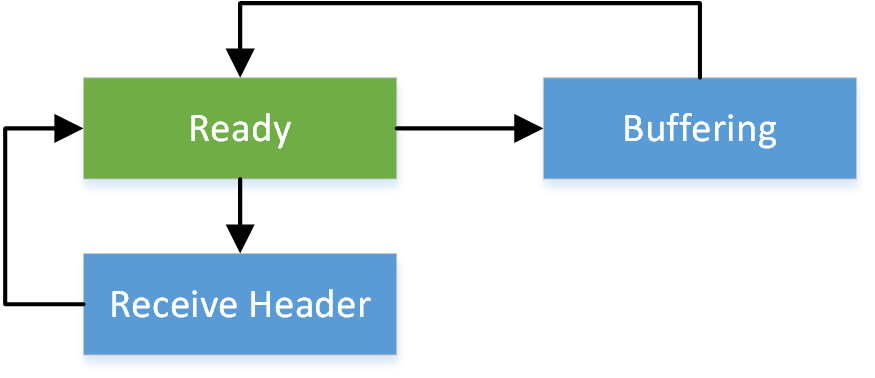
\includegraphics[width=0.5\textwidth]{figures/cncMachine/communications_simple.png}
				\caption{Communications States}
				\label{fig:comms-states}
			\end{figure}
	
	The Communications program, shown in Figure ~\ref{fig:comms-states}, has the role of communicating with the PC to populate the command buffer with the output of the PCs optimization stage using the network interfaced designed in Section ~\ref{sec:network}.

	
			\begin{description}
				\item[Ready] The Communications program does nothing.
				\item[Receive Header] The Communications program initializes the Ethernet socket interface and then starts requesting a header. If no header is received it continues to request until a valid one is received, in which case it returns to the Ready state and tells the Governor it is done.
				\item[Buffering] In the Buffer state, the Communications module requests commands and populating the command buffer, ensuring it doesn't overwrite data that hasn't been executed by motorControl yet. Once it has received the amount of commands specified in the header, it returns to the Ready state and informs the Governor it's done.
			\end{description}
			
		Please see Figure ~\ref{fig:communicationsStates} in Appendix ~\ref{ch:PLC-flowcharts} for more detailed information on how the Communications Program operates.


\subsection{motorControl}

			\begin{figure}[h]
				\centering
				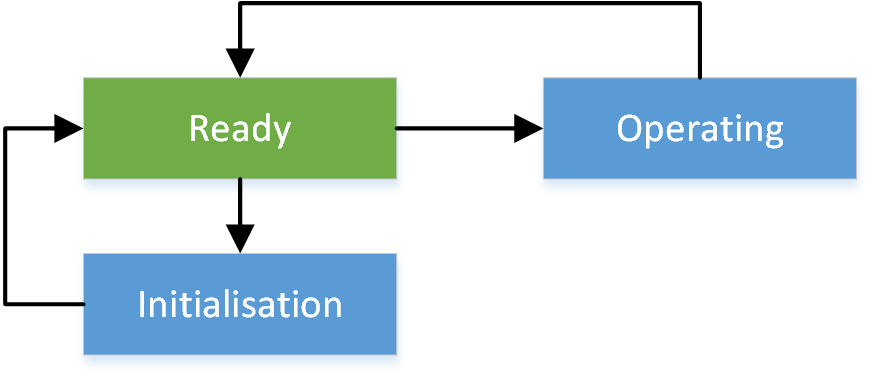
\includegraphics[width=0.5\textwidth]{figures/cncMachine/motorControl_simple.png}
				\caption{motorControl States}
				\label{fig:motorcontrol-states}
			\end{figure}
	
	The motorControl program, shown in Figure ~\ref{fig:motorcontrol-states}, has the role of controlling the electromechanical hardware via the AMCI 3401 module and the PLC Embedded I/O. 
	
			\begin{description}
				\item[Ready] The motorControl program does nothing.
				\item[Initialisation] The motorControl program runs its initialisation routine, which involves configuring the AMCI 3401 stepper motor modules and then running both motors in both directions until the limit switches are activated. This locates the boundaries of the CNC machine respective to the existing state of the motors, and allows the program to locate a centre point and set that to be the (0,0) point. It then returns to the Ready state and informs the Governor it's done.
				\item[Operating] In the operating state, motorControl reads the commands in the buffer and executes them. 'Move' type commands involve moving to a required point at a fixed velocity while retracting the drawing head. 'Draw' type commands involve extended the drawing head and then running a sampled velocity profile at the rate set in the header file.
			\end{description}
			
		Please see Section ~\ref{sec:PLC-flowcharts-motor}in Appendix ~\ref{ch:PLC-flowcharts} for more detailed information on how motorControl and the AMCI 3401 module operate.

	\subsubsection{Stepper Motor Direction Management}	
	\label{sec:stepperdirectionmanagement}
			Empirical observation of the AMCI 3401 modules in operation showed a significant delay (in the order of 2-3 seconds) between distinct commands. This delay was also present when switching between the Manual Move Clockwise and the Manual Move Counterclockwise commands. In contrast, changing the programmed speed while in either manual move state had negligible delay.
			
			This behaviour was a significant issue since the optimized velocity profiles require both axes to track the commands within the period of sampling (in the order of 30-150ms) to follow the required path and as such a 2-3 second delay would prevent proper operation.
			
			To overcome this problem, the DoodleBot controls the direction output via the PLC embedded DC output pins 0 and 1. Direction control is hence done  through code in the motorControl program rather than allow the AMCI 3401 modules to handle the task. The modules will just be constantly run with 'clockwise' commands and assume they are never making the direction switch. 
			
			To continue using Absolute Moves, this also required extra code to keep track of the current position.
			
			Please see Appendix ~\ref{sec:PLC-flowcharts-pos} for more detail on how this part of the code works. A flowchart of this code can be found in Figure ~\ref{fig:Direction and Positional Tracking}.
			
	\subsubsection{Draw Mode Initialisation - Dummy Commands}
			Section ~\ref{stepperdirectionmanagement} identified a method to eliminate the effect of the Stepper Motor lag between distinct commands by always commanding the AMCI 3401 modules to run in the same direction and controlling the Direction separately. There was however, still the initial lag when starting a velocity profile.
			
			To overcome this every velocity profile is padded with some 'dummy' commands that have the machine travel back very slowly and forth at the sample rate  (in the order of single steps), which means there is no noticeably drawn content. The command lag will means only these 'dummy commands' are skipped and ensures that when the real commands are processed they aren't skipped.
			
			At a sampling time of 40ms, 25 'dummy commands' were required to eliminate the module skipping 'real' commands.

	\subsubsection{Overcoming AMCI 3401 Internal Timer Issues}
			After experiencing some issues during testing, a conjectured model of the AMCI 3401's internal workings was made: "A new programmed speed is received by the AMCI 3401 while in a clockwise movement state. The programmed speed is the frequency of step pulses to produce per second and this translates to a period in between pulses. The AMCI 3401 then sets a timer to 0 and counts one period before producing the first step."
			
			The important note of this model to effect is that the internal timer is reset on every new programmed speed received. This assumption was made due to the observed effect of programmed speeds below a certain threshold not causing any movement. The model would explain the issue since if the period of step output is greater than the sample period, the timer would never actually approach the time in which it generates its first step and would keep resetting back to 0 with every command.
			
			Thus if this model were correct, there would be a minimum programmed speed threshold for the stepper modules to be able to move at all equal to $Speed_{minimum} = 1000ms/Sample_{time}$. So at 40ms, the minimum speed threshold would be 25 steps/second.
			
			To alleviate this effect, the DoodleBot has code that sets any code below this threshold to be equal to the minimum speed (except where the axis is completely stationary). 
			
			Further testing confirmed significantly better results. There are theoretical inaccuracies caused by the fact any velocity information below the threshold is lost, however this is significantly outweighed by the significant improvements found by using this fix. 

\subsection{checkLimitSwitch}
	The checkLimitSwitch program is run in a Periodic Task of 10ms and monitors the four limit switches. Upon detecting a rising edge (ie, the machine has hit the end of its range of motion) it alerts the motorControl program. If the motorControl program is in Operating Mode, it'll trigger an emergency stop and halt all operation.
	
	Please see Section ~\ref{sec:PLC-flowcharts-limit} in Appendix ~\ref{ch:PLC-flowcharts} for more detail on how checkLimitSwitch operates.

\section{User Interface}
One of the design criteria for the DoodleBot was that the product was easy for a non-technical user to operate. An obvious requirement for this to be the case was the creation of a Graphical User Interface (GUI) which abstracted the URBS curve generation, image filtering and optimisation processing from the user. This would instead give the user an experience which was intuitive and similar to previous experiences with computer programs. To this end, a GUI similar in design to most drawing programs was developed.
Given that the user would be interacting with a simple interface, the pipeline for the generation of printing instructions was automated. This was achieved with a Java program, modules of which formed the GUI, interface with MATLAB\textsuperscript{\textregistered} and the server to the DoodleBot.
\subsection{Java Program}
The Java code is the backbone that interfaces between the separate modules of the host system. These modules are the Graphical User Inferface (GUI), the MATLAB\textsuperscript{\textregistered} optimisation, the MATLAB\textsuperscript{\textregistered} image processing and the profile server. Each module has a separate program class and thread. The result of the class interactions generates a desired sequence of velocity profiles to be enacted by the CNC machine. A thread is a term used to describe a linear process happening in parallel with multiple other processes. The general outlay of the components of the system can be seen in Figure\ref{fig:javaOverview}


\begin{figure}[htbp]  
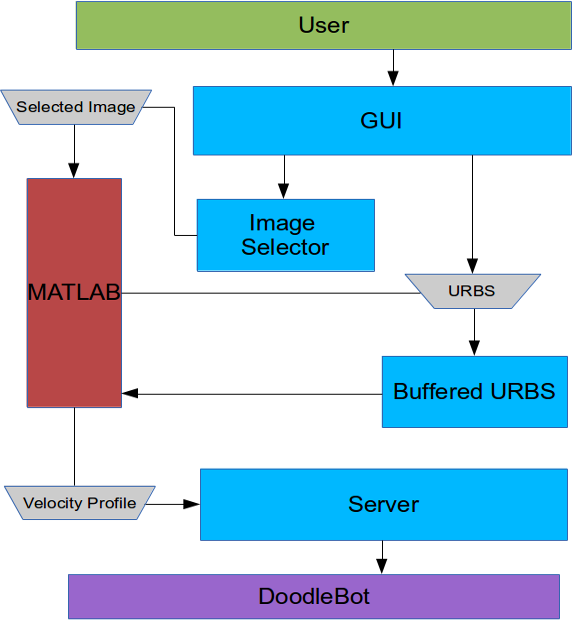
\includegraphics[width=\textwidth]{figures/implementation/humanMachineInterface/systemDiagram.png}
\caption[Human Machine Interface System Diagram]{This diagram demonstrates the interconnection of the components of the computer program that enables the user to interface with the DoodleBot. The components in BLUE represent Java modules. The component in RED represents the MATLAB\textsuperscript{\textregistered} interface.
\label{fig:javaOverview}}
\end{figure}

The overall system consists of separate program threads for each module. This allows processing operations to run in the background while the user can continue to interact with the program. User input occurs through the GUI program thread with direct input and input via selected images. The results are added to a buffer of curves which are displayed to the user. When the user is satisfied with the contents of the buffer they can order the program to print. This moves the buffered curves into a processing queue on the MATLAB\textsuperscript{\textregistered} interface program thread. This move means that the buffered curves will all be processed and printed. Curves are processed into velocity profiles with the optimisation algorithm in MATLAB\textsuperscript{\textregistered} and then loaded into the server program thread, which communicates the desired curves with the DoodleBot.
\section{MATLAB\textsuperscript{\textregistered} Image Processing}

\chapter{Performance and Testing}

\input{chapters/performance/outline}
\section{Path Discretisation}
The discrete approximation of the path was performed in order to solve for the time-optimal trajectory of the DoodleBot. The approximation of the problem spreads speed choking points of the path out over a greater path length, which intuitively leads to longer traversal times. The traversal time for a range of path discretisation lengths can be seen in Figure \ref{fig:sDivisions}. The overall trend for the traversal time is an exponential decay to a constant value which corresponds to the optimum traversal time for the true solution. This value is reached consistently at approximately 80 path divisions. As such, 80 divisions forms the lower bound on the number of discretisations for an acceptable approximation. As the number of control points increases, so too should the number of discretisations, as the number of control points a curve contains correlates linearly with the complexity of the curve and linearly with the number of possible limiting axis switching points.
An interesting effect and something that showcases a flaw in the discretisation approximation can also be seen in Figure \ref{fig:sDivisions}. Note the repetitive stutter pattern in the shape of the decaying completion time. Note also, that the completion time for some of the stutters falls below the convergent minimum possible value. This effect is caused by the path discretisation approximating the constraints of the curve as though the system can be traversed faster than the true constraints allow. This occurs due to the discrete switching of the restrictions extending a section that allows fast travel for longer than that section actually exists. This extension exists even though maximums are taken of the magnitude of the path derivatives, as discussed in previous sections. The combinations of the signs and magnitudes of the path derivatives mean that something that the algorithm picks as a constraint, might not actually be the true constraint for the entire discretisation. This bleeding specifies that the DoodleBot should be speeding up when, in order to obey the constraints, it should be slowing down. Thus a lower number of path divisions may result in a trajectory which is impossible for a mechanism with the limits on acceleration specified to traverse. This effect is possible at 80 path divisions and even higher, but is can be seen from the decaying oscillation that the effect becomes a smaller problem at higher divisions. The effect is also mitigated by the fact that the hard limits of the motor are not the limits that are set for the solution, but rather a smaller soft limit is requested. This allows the small trespasses on the maximum limits to be followed by the motors without error.


\begin{figure}[htbp]  
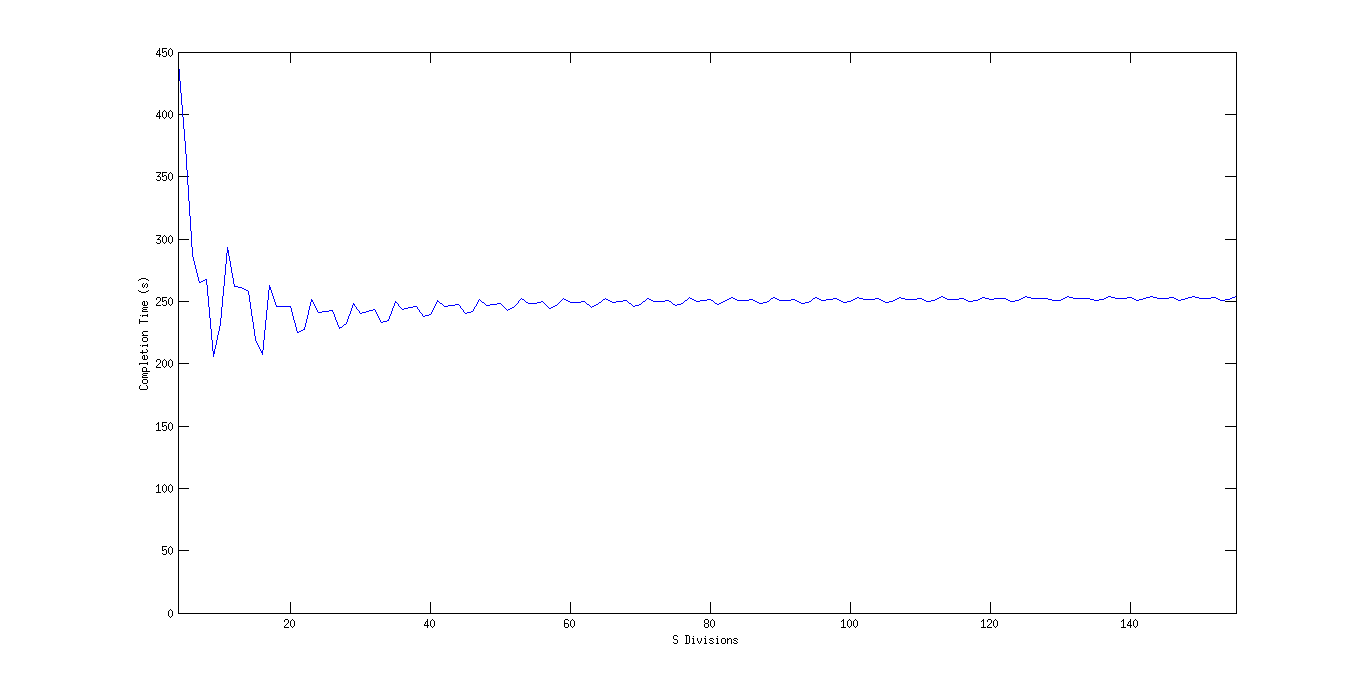
\includegraphics[width=\textwidth]{figures/performance/sDivisions.png}
\caption[Trajectory completion time for a range of path discretisation lengths]{Trajectory completion times for a range of path discretisation divisions
\label{fig:sDivisions}}
\end{figure} 

A limitation of the solution process that prevents the solver from simply solving for an arbitrarily large number of discretisation steps is the fact that the solver becomes numerically unstable at a threshold of around 1500 discretisation intervals, meaning that solutions are often not possible past this value. A second reason which forms a limitation when one considers the desire to minimise the length of the whole printing process is the exponential growth of computation time as the number of discretisation intervals increases. The DoodleBot processes the input upon the request of the user to print a series of curves. Ideally, the processing time of the curve optimisation is not the limiting factor in the printing process. However with large discretisation values, the processing time balloons out to values such as 384 seconds, or about 6 minutes per curve. This means that a tradeoff between the computation time and optimality must be made. Figure \ref{fig:sDivTime} demonstrates the processing time increase with the number of divisions. The average traversal time for a curve on the DoodleBot hardware is about 8 seconds at the optimal torque limits. This approximately corresponds the value that was set for the DoodleBot's default number of path discretisations, at 200. This level of discretisation gives a good approximation of the optimal solution without stretching the acceleration constraints. This value also remains below the average curve execution time, so that curves are processed faster than they are traversed.

\begin{figure}[htbp]  
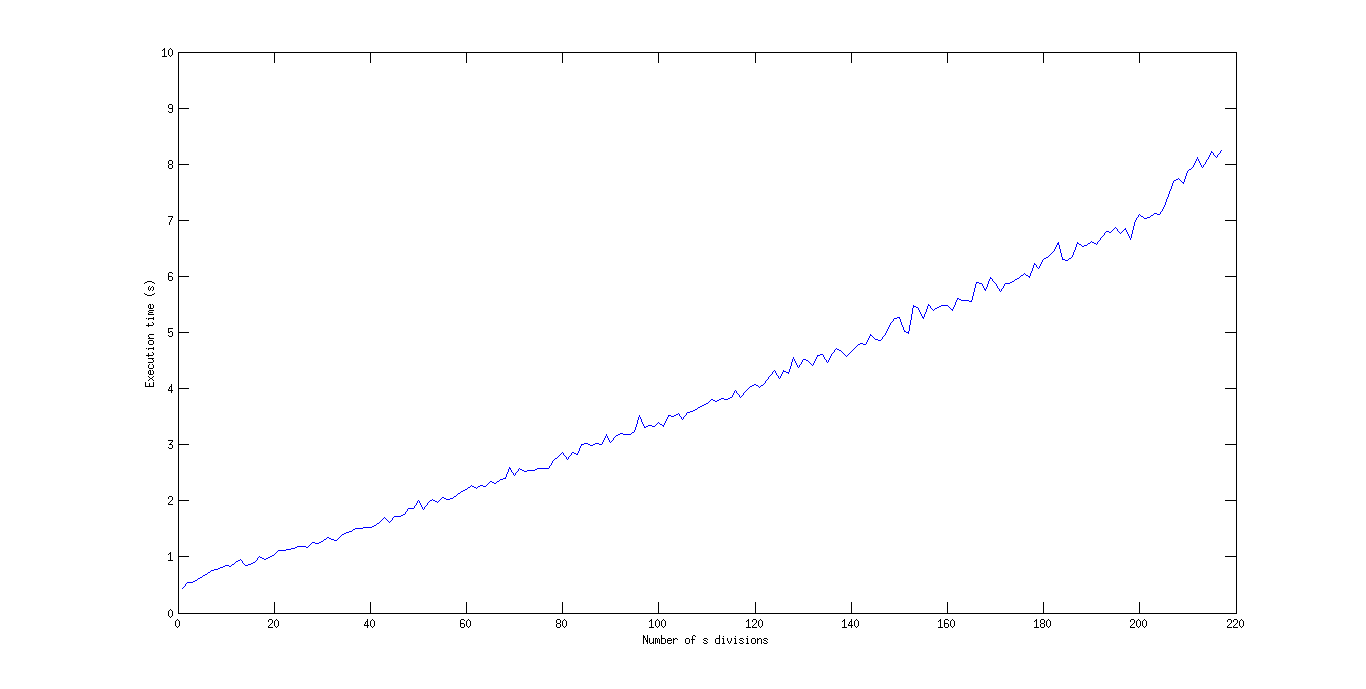
\includegraphics[width=\textwidth]{figures/performance/sDivTime.png}
\caption[Processing time for a range of path discretisation lengths]{Processing time for a range of path discretisation lengths
\label{fig:sDivTime}}
\end{figure} 



\section{Sample Time}
\label{ch:performance-sampletime}
%A bottleneck on the accuracy of the final image is the amount of error introduced by the sampling of the velocity profile produced by the solution of the time-optimal control problem. Sampling error is an unavoidable result of a digital system following a given profile. Thus there is a limit on the accuracy of a digital system, especially one which uses integration in order to achieve an outcome. The smallest amount of error will magnify until the result is quite different from that which is desired. Since a digital processing device can only direct an integrating process at a limited rate, sampling errors will accumulate over time and cause the image to become inaccurate. In the case of the DoodleBot, the measured placement of the initial position at the initialisation of a trajectory resets the integration error and as such the error can only accumulate over a single curve. The effect of operating at differing sample periods can be seen in Figure \ref{fig:timestep}.

The Optimisation module is able to produce continuous velocity profiles that perfectly track the required URBS, however the PLC and network interface require discrete sampled packets, and so the velocity profiles need to be discretized. This is inherently an approximation that will lose accuracy.
\begin{figure}[hp]
\includegraphics[width=\textwidth]{figures/performance/timestep.png}
\caption[Comparison of differing velocity sampling frequencies]{A comparison of velocity sampling periods. From top left to bottom right; 1) 20ms 2) 40ms 3) 80ms 4) 120ms 5) 150ms 6) 200ms
\label{fig:timestep}}
\end{figure} 

\begin{figure}
\centering
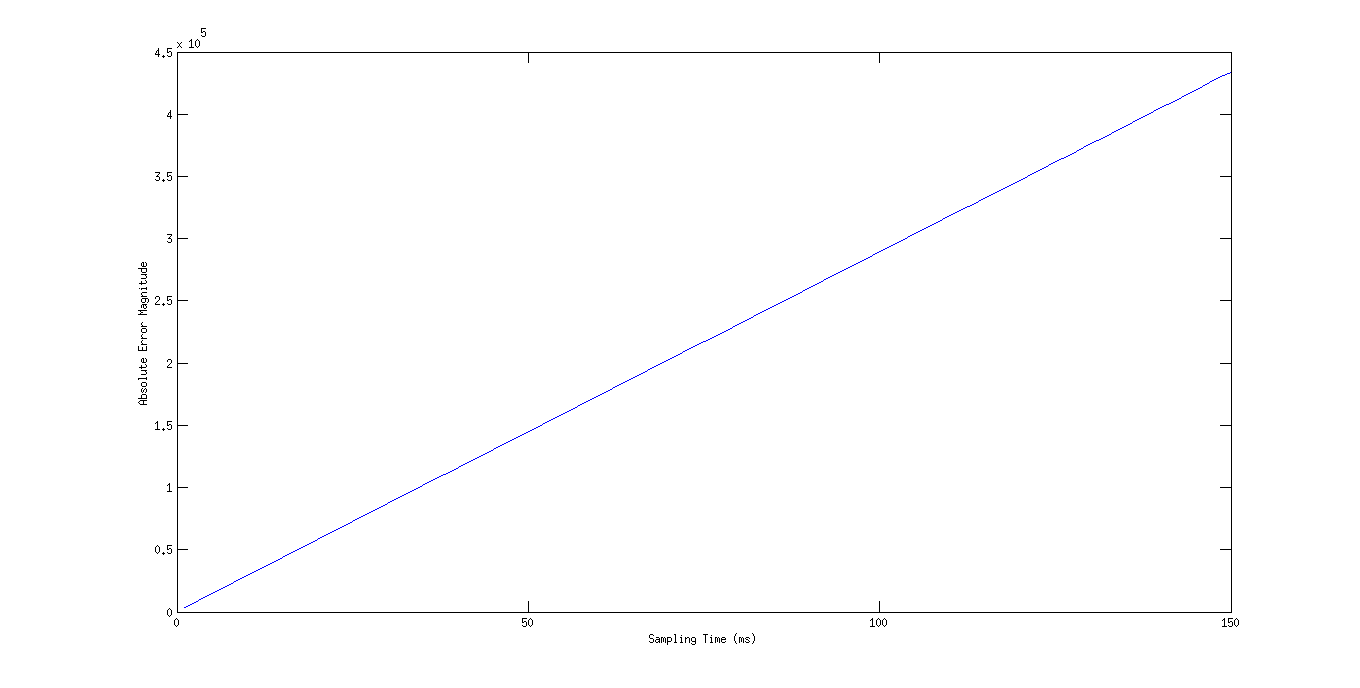
\includegraphics[width=0.8\textwidth]{figures/performance/tStep.png}
\caption[Plot of error magnitude against velocity sampling period]{Error magnitude against velocity sampling period, where the error is calculated to be the distance between the original curve and the sampled curve}
\label{fig:tStep}
\end{figure}  

Figure ~\ref{fig:tStep} shows a chart of the error in the image verses the sampling time, where the error is the deviation between the sampled curve and the original curve summed for a certain number of samples across the length of the curve. The chart shows that as the sampling time drops  the error reduces linearly.

However in the real system, there are minimum constraints on how low the sampling period can go. The sample rate cannot be lower than the time it takes for the network interface to buffer more commands and it cannot be lower than the time it takes for the PLC to process the command and then implement it on the stepper motors, or whole commands will be skipped. 

Another major effect of lower sampling rates becomes apparent in Figure ~\ref{fig:timestep}. As the sample time reduces from 200ms to 40ms, there is a clear improvement in the accuracy of the image, as the simulated results would suggest. However, when the sampling time is reduced to 20ms the error actually increases significantly. 

\begin{center}
\centering
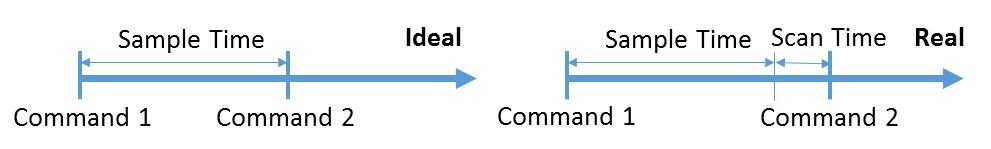
\includegraphics[width=0.6\textwidth]{figures/performance/images/periodscan.jpg}
\captionof{figure}[Sample time inaccuracy]{Real vs ideal behaviour of PLC code sample time}
\label{fig:periodscan}
\end{center}

This unexpected error with lower sample times is likely due to how accurately the PLC is actually able to operate at the specified sample time. Figure ~\ref{fig:periodscan} shows a real vs ideal scenario on how sample time can vary. In the ideal scenario, as soon as the internal counter reaches the sample time a command will be executed and the timer reset. In reality, the PLC has to scan through the code one line at a time and might take some extra time before executing the command and resetting the internal timer. This means that the system will run a single command for longer than it should. 

The PLC scan times vary from 0.1ms-1.5ms, and hence cannot be compensated for in the code. Since the scan times don't seem to be effected by sample times, lower sample times lead to a higher proportional error in the real vs specified sample time. This creates a trade off between inherent error from approximation by lowering the scan times and minimizing the proportion of error between the real and ideal scan times by increasing the scan times. Experimentation found $40ms$ or $25Hz$ to be the best compromise between these two trade offs. 



 



%Two effects are at play in the alteration of the sampling period. A limit exists on the lowering of the sampling period below the time required for the controller to undergo one iteration of the control loop. Beyond this point variance in the loop timing can weight some commands noticeably more than others, even to the point where commands begin to get skipped or are not active for a long enough duration to have an effect. This causes the type of distortion in the final image that can be seen in the top left profile in Figure \ref{fig:timestep}. The second effect of the sampling period on the accuracy of the output image is that an increase in the sampling period corresponds to a larger approximation of the correct velocity profile. The looser an approximation becomes, the greater the integral error will become over the length of the curve. Figure \ref{fig:timestep} demonstrates this effect. As the as the sampling period increases the amount of error becomes progressively greater. Figure \ref{fig:tStep} demonstrates that the level of error in the final image is linearly correlated with respect to the sampling period.

%It is evident that the best policy is to decrease the sample period until just before the limits of the control loop manifest. The DoodleBot was found to perform best at a 40ms sampling period, or at 25Hz.
\section{Acceleration Constraints}
In order to achieve the goal of minimising the time that the DoodleBot takes to complete a curve, the acceleration limits must be considered. These limits are the main design parameter that has a direct impact on the completion time for all curves. Figure \ref{fig:maxAccel} demonstrates the effect that increasing the acceleration limits has on the completion time for a given trajectory. It becomes clear that it is desirous to increase the acceleration limits as far as possible. However there are physical limits which degrade performance past certain thresholds.

\begin{figure}[htbp]  
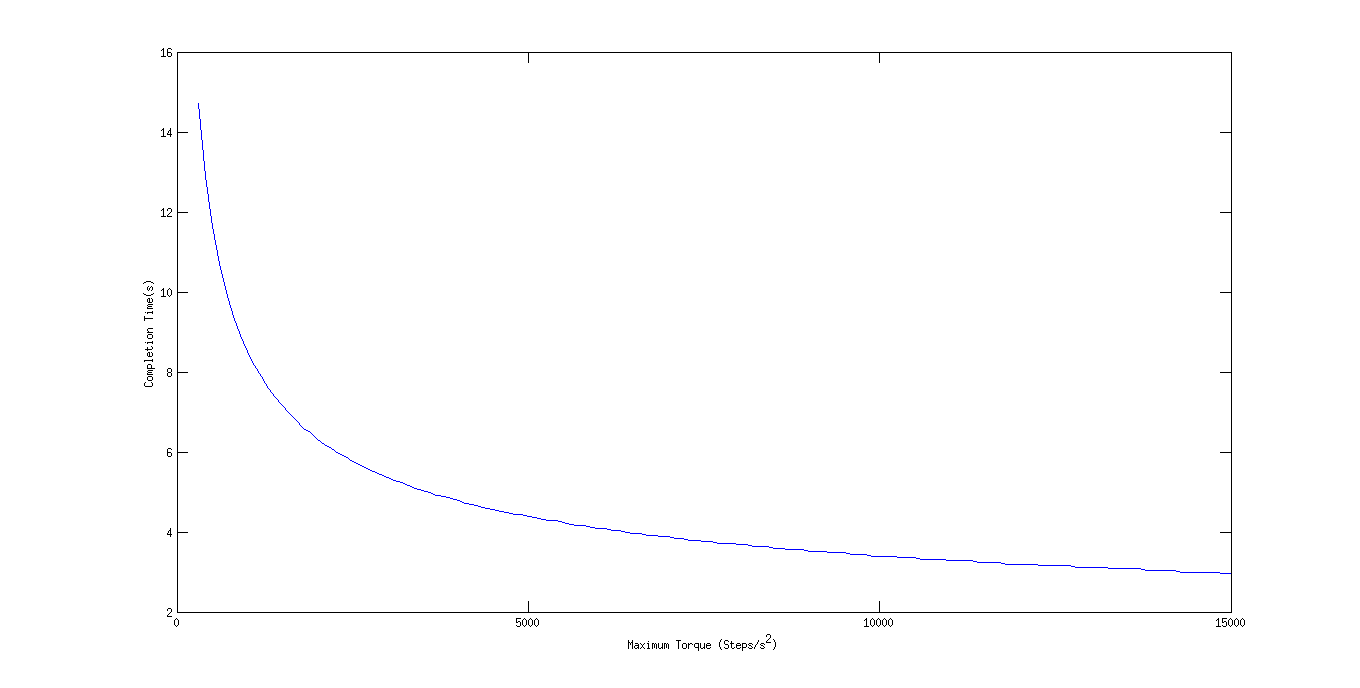
\includegraphics[width=\textwidth]{figures/performance/maxTorque.png}
\caption[Trajectory completion time against maximum acceleration limits]{Trajectory completion time against maximum acceleration limits
\label{fig:maxAccel}}
\end{figure}  	

The plant model derived for the DoodleBot allowed us to consider that for given acceleration limits the plant maps input to output perfectly. This allows us to give commands in open loop without fear of inaccuracy as long as we can guarantee that the acceleration limits will not be exceeded. As the plant is worked closer and closer to its limitations the perfect mapping of input to output begins to break down, resulting in unavoidable inaccuracy. There are two types of behaviour which can occur whilst close to the acceleration limits. 

The first is a catastrophic synchronisation failure between the step commands and the movements of the stepper motor. If the motor falls out of sync, step inputs essentially become random perturbations on the motor spindle. This means that the motor gains no net torque from the power input into the stepper coils, as the direction that the spindle is pulled is no longer in necessarily in the direction of desired travel due to the lack of synchronicity. The step commands come faster and faster and the motor spindle will simply vibrate in place, as the spindle cannot hope to accelerate to catch back up to the step rate. This type of failure is obvious and results in a complete failure to match the desired curve.

The second type of failure is a missed step, which occurs when a transient or other load causes the motor to fail to achieve the correct position by the time that the controller progresses to the next step. For a few subsequent steps, the motor continues under its own momentum with the step input of the controller assisting or hindering its progress at random. If the motor does not completely fall out of sync, the pulses will eventually realign themselves with the motor and the motor will continue without a total failure. These missed steps are not detected by the controller and will become a permanent offset for the rest of the motor's movement until there is a complete readjustment of the mechanism. Indeed these missed steps happen over a matter of milliseconds, so it is hard for human operators to tell when this kind of error occurs.

Higher accelerations also amplify the effect of the sample time error found in Section ~\ref{ch:performance-sampletime}.

A range of curves run at differing acceleration limits can be seen in Figure \ref{fig:accelLimits}.
	
\begin{figure}[htbp]  

\includegraphics[width=\textwidth]{figures/performance/accelLimits.png}
\caption[Comparison of differing acceleration constraints]{A comparison of the results of differing acceleration constraints. From top left to bottom right; 1) $1000\text{ steps}/s^2$ 2) $3000\text{ steps}/s^2$ 3) $5000\text{ steps}/s^2$ 4) $15000\text{ steps}/s^2$
\label{fig:accelLimits}}
\end{figure}  	

Measuring the accuracy of differing acceleration limits and attempting to notice the effect of step skipping is a complicated by the fact that lower acceleration limits result in a longer traversal time. This longer traversal time means that the velocity profile sampling has a higher equivalent density along the surface of the same curve. This results in better performance when the curve is traversed at a slower rate. Thus efforts to measure the accuracy of the mechanism under different acceleration constraints can be confounded. The limits on acceleration also depend on various factors that can change with time such as; the total load on the armature, friction at points along the axis, voltage supply fluctuations and a myriad of other possibilities.

For this reason it is sound practice to leave a solid buffer between the maximum measured acceleration limits of the device and the constraints given to the optimisation algorithm in order to allow for robustness to error. For the DoodleBot, this level was set to be $1000\text{ steps}/s^2$ as a default, though good performance could be obtained at higher acceleration limits with calibration.
	
\section{Image Interpolation}
Measuring the strength of the image interpolation algorithm objectively is difficult. This also makes the design and improvement of filters a difficult process, as a filter scheme which seems to work well for one image will not work well for another. The field of computer vision is one that attempts to deal with these problems, but a rigorous implementation of algorithms within this field was not the main focus of our implementation. Our objective was to create a filtering system which gave a reasonable and recognisable output for any given input and as such a very general and robust edge capturing algorithm was designed. Arguably the best way to measure the performance of the algorithm is to compare its effectiveness objectively against a range of different input images. A comparison of a selection of inputs and outputs can be seen in Figure \ref{fig:imageInterpolation}.

\begin{figure}[htbp]  
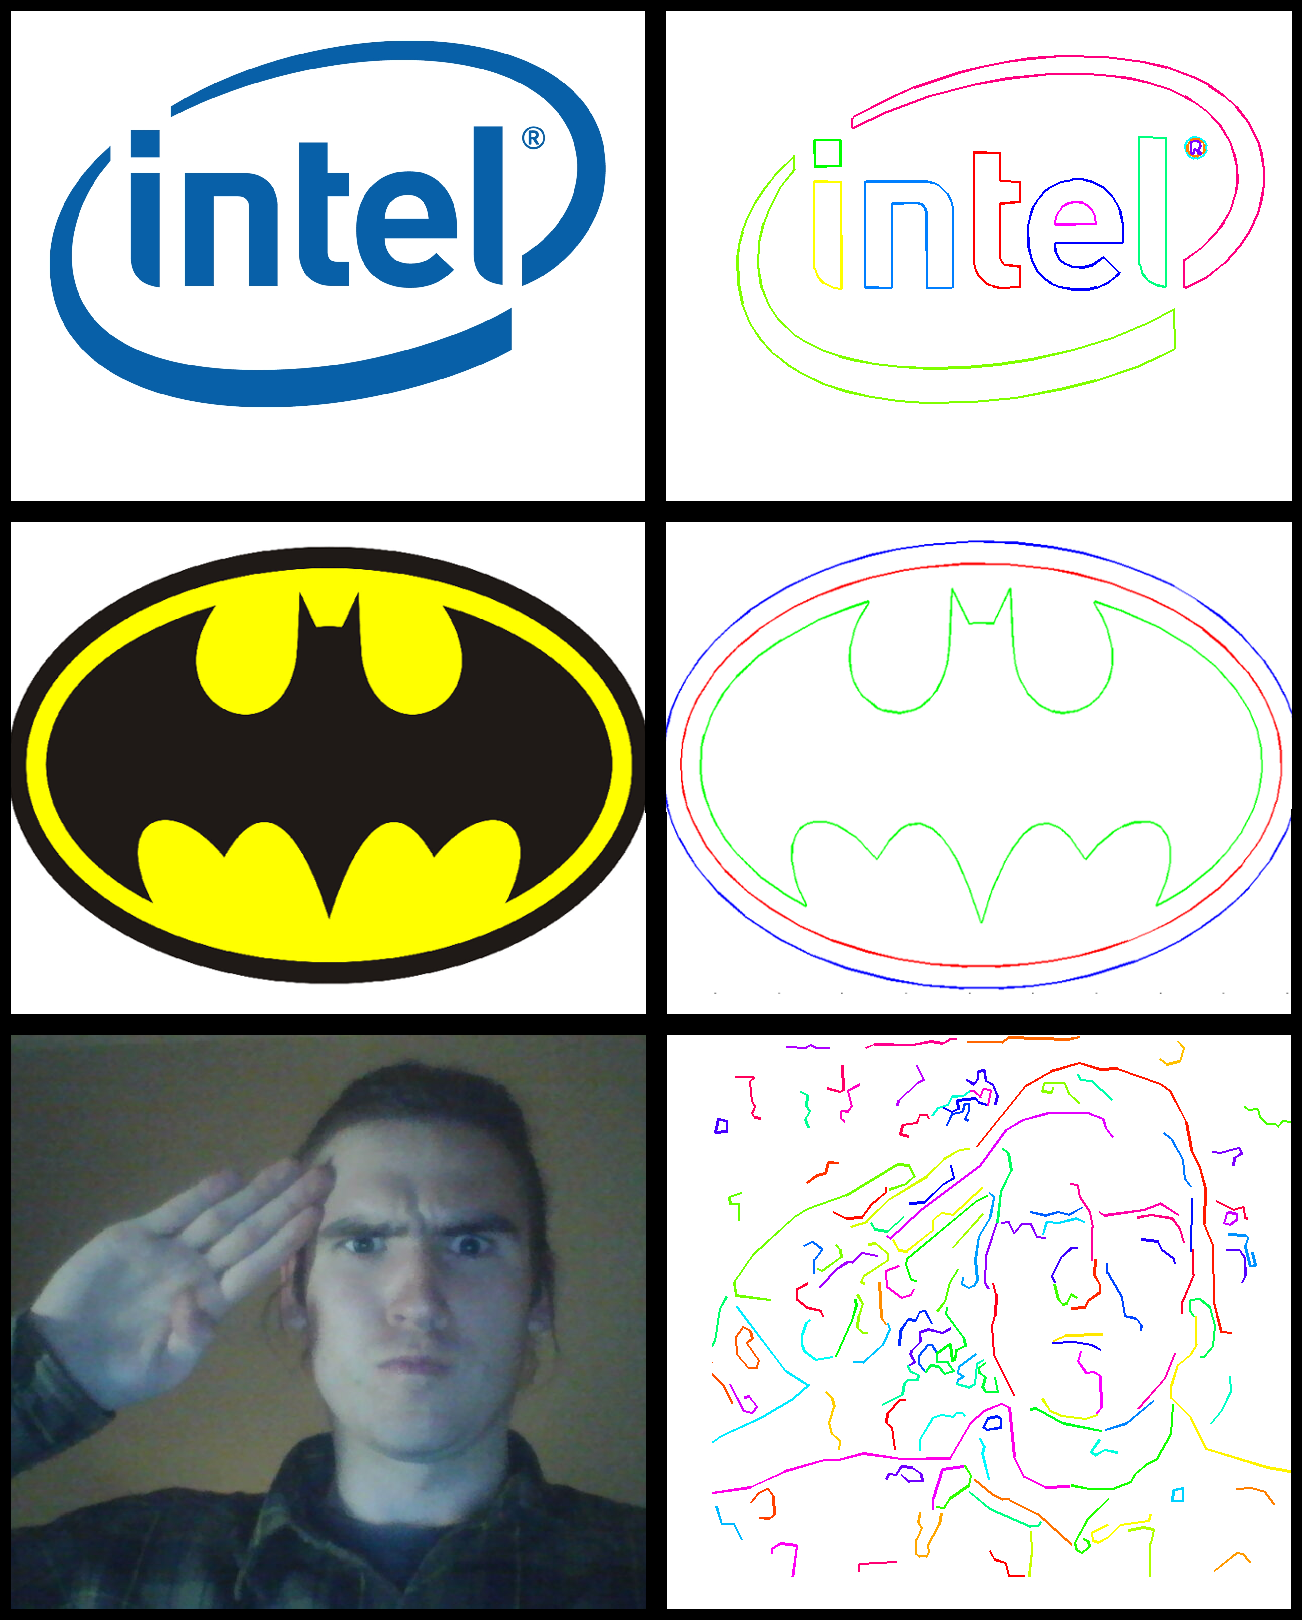
\includegraphics[width=\textwidth]{figures/performance/imageInterpolation.png}
\caption[Examples of image interpolation performance]{Examples of image interpolation performance. LEFT: Image before processing. RIGHT: Plot of the curves extracted from the image.
\label{fig:imageInterpolation}}
\end{figure}

When there are obvious lines to be found, the image filter does an excellent job of finding those lines and composing the image out of them. However, in more complex images such as the colour photo of a face, noise abounds and the many edges are detected in the image. This problem is one that remains generally unsolved in image filtering and arguably there is no correct mapping from an image to a set of contours. Within respect to the intended purpose of the algorithm, simple images or vector drawings are easily imported and are represented very well by the filter. Complex images will have mixed results, but the general gist of the image will be conveyed.



\begin{appendices}
\chapter{URBS Weight Derivation}
The following \cite{website:nurbsExplain} gives a series of derivations of the general case of the weights for URBS splines up to the third order.
In general;
\begin{align*}
W^d_{i}(s) &=   \frac{s - K_i}{K_{i+d} - K_i}W^{d-1}_{i}(s)  +  \frac{K_{i + d + 1} - s}{K_{i + d + 1} - K_{i+1}}W^{d-1}_{i+1}(s)\\
W^0_{i}(s) &= \begin{cases}
   1 & \text{if } K_i \leq s < K_{i+1} \\
   0 & \text{otherwise}
  \end{cases}	
\end{align*}

Using this recursive formula, we can build up results for first order URBS given $K_i \leq s < K_{i+1}$;

\begin{align*}	
W^0_{i-2}(s),W^0_{i+1}(s), W^0_{i-1}(s) &= 0\\
W^0_{i}(s) &= 1 
\end{align*}

Second order;

\begin{align*}	
W^1_{i} &= \frac{s - K_i}{K_{i+1} - K_i}W^0_{i}(s)  +  \frac{K_{i + 2} - s}{K_{i + 2} - K_{i+1}}W^0_{i+1}(s)\\
	 &= \frac{s - K_i}{K_{i+1} - K_i}\\
	 \\
W^1_{i-1}(s) &=   \frac{s - K_{i-1}}{K_{i} - K_{i-1}}W^0_{i-1}(s)  +  \frac{K_{i + 1} - s}{K_{i + 1} - K_{i}}W^0_{i}(s)\\
	&=\frac{K_{i + 1} - s}{K_{i + 1} - K_{i}}
\end{align*}

Third order;

\begin{align*}
W^2_{i}(s) &= \frac{s - K_i}{K_{i+2} - K_i}W^1_{i}(s)  +  \frac{K_{i + 3} - s}{K_{i + 3} - K_{i+1}}W^1_{i+1}(s)\\ 
	&=   \frac{s - K_i}{K_{i+2} - K_i}\frac{s - K_i}{K_{i+1} - K_i}\\ 
	&= \frac{(s - K_i)^2}{(K_{i+2} - K_i)(K_{i+1} - K_i)}
\end{align*}
\begin{align*}
W^2_{i-1}(s) &= \frac{s - K_{i-1}}{K_{i+1} - K_{i-1}}W^1_{i-1}(s)  +  \frac{K_{i + 2} - s}{K_{i + 2} - K_{i}}W^1_{i}(s)\\ 
	 &= \frac{s - K_{i-1}}{K_{i+1} - K_{i-1}}\frac{K_{i + 1} - s}{K_{i + 1} - K_{i}} +  \frac{K_{i + 2} - s}{K_{i + 2} - K_{i}}\frac{s - K_i}{K_{i+1} - K_i}
\end{align*}
\begin{align*}
W^2_{i-2}(s) &= \frac{s - K_{i-2}}{K_{i} - K_{i}}W^1_{i-2}(s)  +  \frac{K_{i + 1} - s}{K_{i + 1} - K_{i-1}}W^1_{i-1}(s)\\
	&=\frac{K_{i + 1} - s}{K_{i + 1} - K_{i-1}}\frac{K_{i + 1} - s}{K_{i + 1} - K_{i}}\\
&=\frac{(K_{i + 1} - s)^2}{(K_{i + 1} - K_{i-1})(K_{i + 1} - K_{i})}
\end{align*}

These weightings define the linear combination of the control points creating a point on the curve;
\begin{align*}
P(s) = \textbf{N}_i^2W^2_{i}(s) + \textbf{N}_{i-1}^2W^2_{i-1}(s) + \textbf{N}_{i-2}^2W^2_{i-2}(s)
\end{align*}

for $K_i \leq s < K_{i+1}$.
%\chapter{Derivation of $s^(t)$ given $\dot{s}^{2}(s)$}
We are given that $\dot{s}^{*2}(s)$ is piecewise linear and continuous. Thus we can determine $\dot{s}^*(s)$ at each of the edges of the piecewise functions. We also have the equality
\begin{align*}
t^*(s) &= \int^s_0\frac{1}{\dot{s^*}(s)}ds
\end{align*} 
The computer algorithm used to extract a profile of $s$ for a given increment of $t$ calculates the total time taken to reach the ends of each of the piecewise sections. A piecewise integration is performed between each of these points in order to obtain a given time increment as follows;
\begin{align*}
\Delta t_k(s) &= \int_{s_k}^s \frac{1}{\sqrt{\frac{\dot{s}(s_{k+1}) - \dot{s}(s_{k})}{s_{k+1} - s_{k}}} u + \dot{s}(s_{k})} du
\end{align*}
This equation gives the increment in time from the border of a piecewise section of $\dot{s}^*(s)$, where $s_k$ is the edge of the border.
Given that we can calculate the value of $t$ at the borders of each of the piecewise function by summing all previous piecewise integrals, we can denote the value of $t$ at the $k$th border as $t_k$ and the value of $s$ at the $k$th border as $s_k$. The border values of $s_k$ can be computed via;
\begin{align*}
s_{k+1} - s_k &= \frac{2\Delta s}{\dot{s}^2_k - \dot{s}^2_{k-1}} \left(\dot{s}_k -\dot{s}_{k-1}\right)
\end{align*}
This bordering value of $s_k$ allows us to compute the increment of $\Delta_s$ past this border for any $\Delta_t$. Hence, we can index a given value of $t$ into the interval where $t_k < t = t_k + \Delta_t \leq t_{k+1}$ in order to obtain the relation
\begin{align*}
s(t) &= \sum_{k=1}^{s_k < s(t_k)} \frac{2\Delta s}{\dot{s}^2_k - \dot{s}^2_{k-1}} \left(\dot{s}_k -\dot{s}_{k-1}\right) + \left(\left(\frac{(t-t_{k})(\dot{s}^2_{k+1} - \dot{s}^2_{k})}{2 \Delta s} + \dot{s}_k\right)^2 - \dot{s}^2_k \right)\frac{\Delta s}{(\dot{s}^2_{k+1} - \dot{s}^2_{k})}\\	
\end{align*}
\chapter{PLC State Machine Detailed Design and Flowcharts}
\label{ch:PLC-flowcharts}

		\section{Intraprogram Interfaces and Global Data}
		The Governor program interfaces with the Communications and motorControl programs via the two global scope variables, \textit{motorControl\_mode} and \textit{communications\_mode} which act as intraprogram interfaces. On each state transition, the Governor sets these variables  to certain values, determining what state to move the other programs into. The other programs can then set these variables to different values, informing the Governor on their own state changes and status which the Governor then uses as state transition conditions. Table ~\ref{table:progaminterfaces} shows the possible values of the intraprogram interfaces. 
		
		\begin{table}[htbp!]
			\begin{tabular}{|c|l|l|l|}
				\hline
				Code & motorControl\_mode & communications\_mode & Set By \\ \hline
				00 & Wait & Wait & Governor \\ \hline
				10 & Initialize & Ready & Governor\\ \hline
				11 & Initialization complete & Header received & motorControl/communications \\ \hline
				20 & Operate commands & Buffer command list & Governor \\ \hline
				21 & All buffered commands complete & Buffering complete & motorControl/communications\\ \hline
				22 & N/A & Buffer full & communications\\ \hline
			\end{tabular}
			\caption{Codes for interface between Governor, Communications and motorControl programs}
			\label{table:progaminterfaces}
		\end{table}
	
		In addition to locally scoped variables, there are also several key global scope variables that are used by two or more program that determine the behaviour and input of the system. These are shown in Figure ~\ref{table:globalvariables}

	\begin{center}
			\begin{tabular}{|l|l|p{10cm}|}
				\hline
				Variable Name & Element & Description\\ \hline
			%Spill over is included as a 'row', so use 4 instead of 2 for multirow
				\multirow{4}{*}{counterCommand} & .counter & Index number of the command currently being operated on by motorControl (also, how many commands have been processed)\\ \cline{2-3}
					 & .pointer & Index of where the command referred to by counterCommand.counter resides in the commandBuffer array\\ \hline
				\multirow{4}{*}{counterBuffer} & .counter & Index number of the command currently being buffered by Communications (also, how many commands have been buffered)\\ \cline{2-3}
					 & .pointer & Index of where the command referred to by counterBuffer.counter resides in the commandBuffer array\\ \hline
				\multirow{8}{*}{commandBuffer[]} & .command\_no & Command number of what the current array element stores\\ \cline{2-3}
					& .type & Determines the command type. 0 is a 'draw' and 1 is a 'move'. \\ \cline{2-3}
					& .x\_speed & For 'draw' operations, determines the X target speed for this sample. For 'move' operations, determines the target position for X to move to. \\ \cline{2-3}
					& .y\_speed & For 'draw' operations, determines the Y target speed for this sample. For 'move' operations, determines the target position for Y to move to. \\ \hline
				\multirow{8}{*}{boundaries} & .X\_CW & The number of clockwise steps from the center until the boundary in the X positive direction\\ \cline{2-3}
					 & .X\_CCW & The number of clockwise steps from the center until the boundary in the X negative direction\\\cline{2-3}
					 & .Y\_CW & The number of clockwise steps from the center until the boundary in the Y negative direction\\ \cline{2-3}
					 & .Y\_CCW & The number of clockwise steps from the center until the boundary in the Y positive direction\\ \hline
				\multirow{6}{*}{header} & .delta\_time & Period of velocity profile samples\\ \cline{2-3}
					 & .no\_commands & Total number of commands to be received and executed on\\ \cline{2-3}
					 & .max\_accel\_x & Max acceleration in the X axis\\ \cline{2-3}
					 &  .max\_accel\_y & Max acceleration in the Y axis\\ \cline{2-3}
					 & .move\_speed\_x & Target speed for 'move' operations in the X axis\\ \cline{2-3}
					 & .move\_speed\_y & Target speed for 'move' operations in the Y axis\\ \hline
			\end{tabular}
			\captionof{table}{Important global scope variables used by multiple programs}
			\label{table:globalvariables}
		\end{center}


\section{Governor}

		\begin{center}
				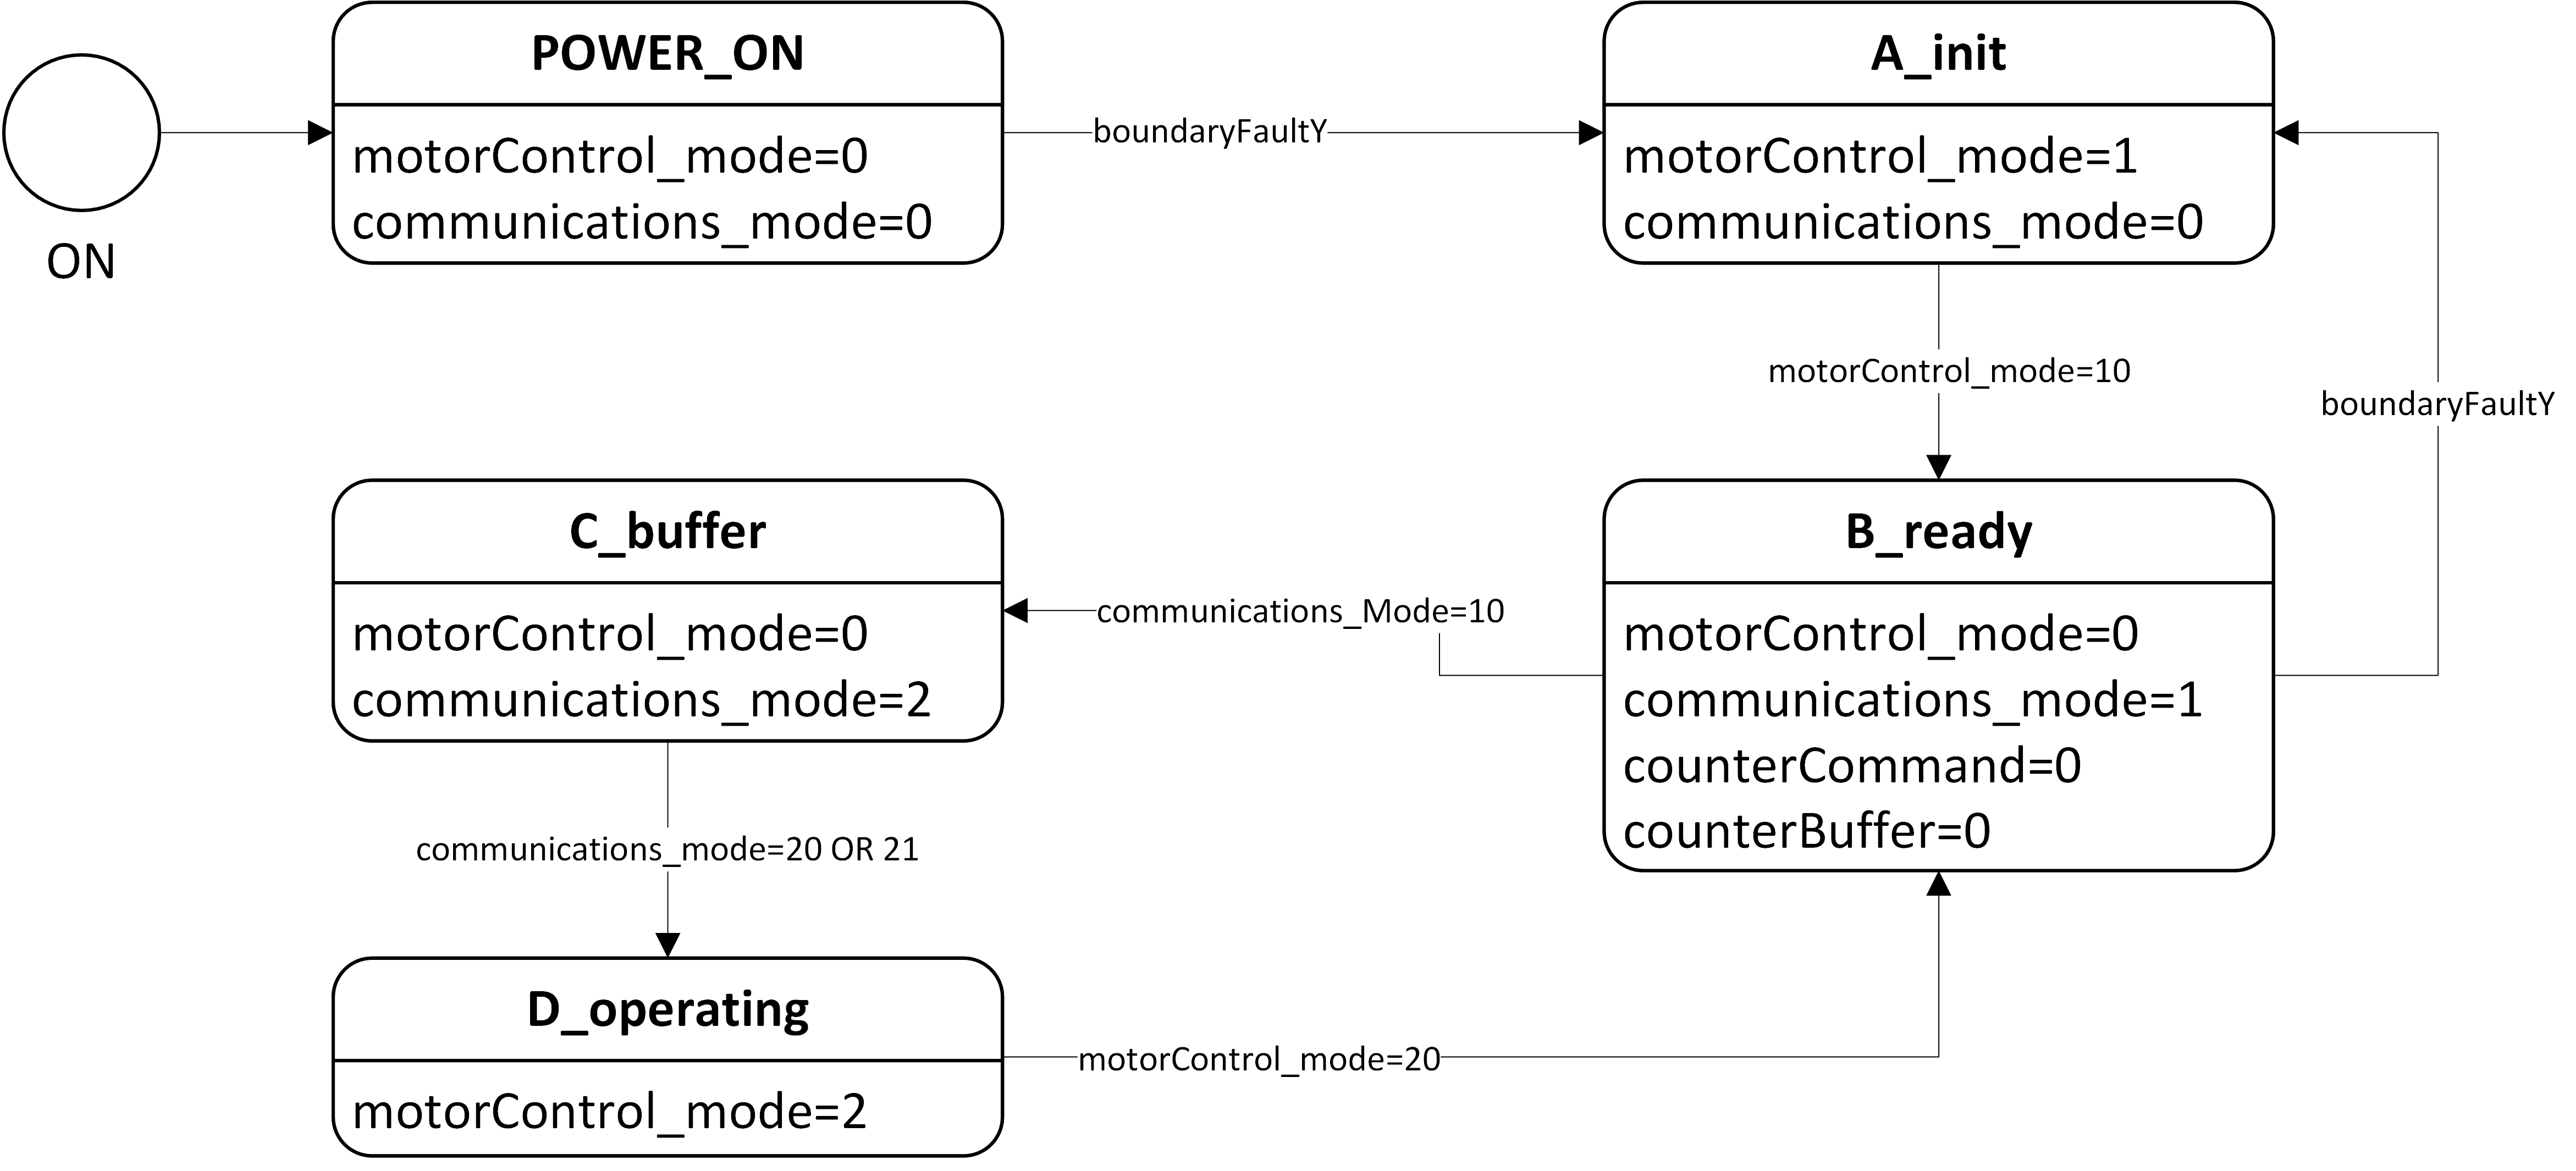
\includegraphics[width=\textwidth]{figures/cncMachine/governor}
				\captionof{figure}{The Governor State Machine}
				\label{fig:PLC-flowcharts-governor}
		\end{center}

\section{Communications State Machine}
\label{sec:PLC-flowcharts-comms}

	\begin{center}
		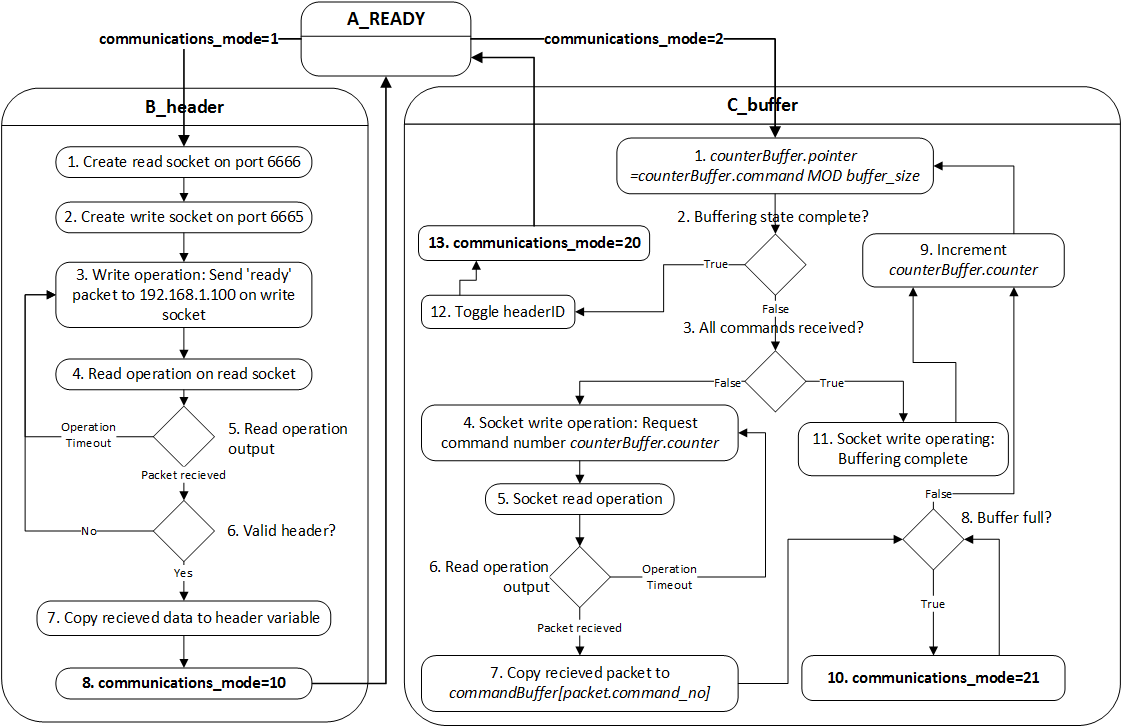
\includegraphics[width=\textwidth]{figures/cncMachine/communications}
		\captionof{figure}{Communications program: States and State Actions}
		\label{fig:communicationsStates}
	\end{center}

\section{motorControl State Machine}
\label{sec:PLC-flowcharts-motor}
	\begin{center}
		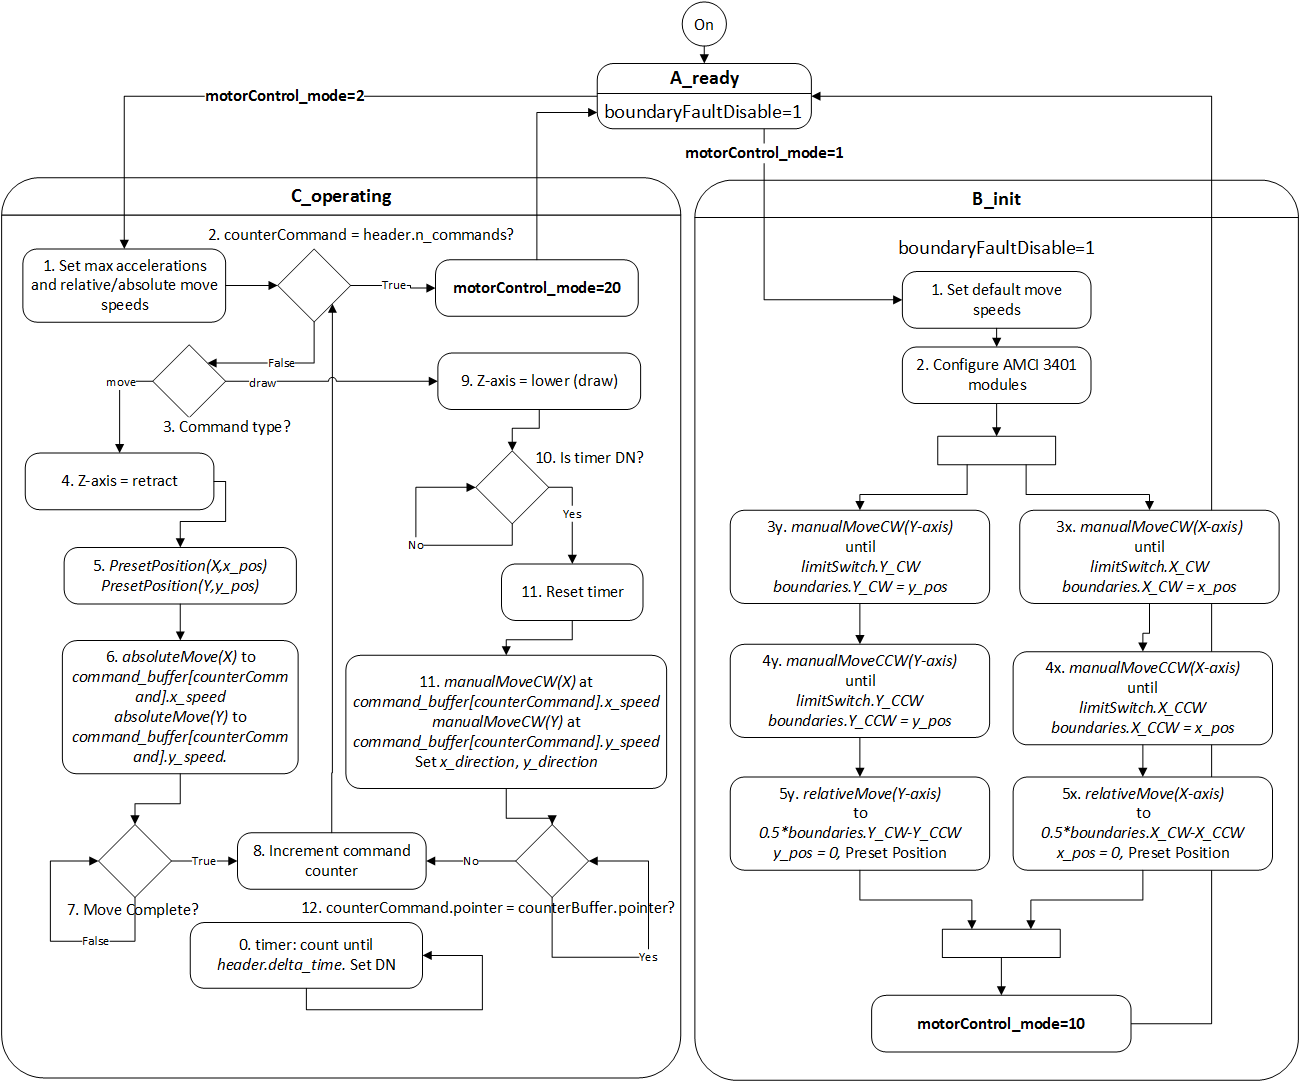
\includegraphics[width=\textwidth]{figures/cncMachine/motorControl}
		\captionof{figure}{motorControl Program: States and State Actions}
		\label{fig:motorControlStates}
	\end{center}

	\subsubsection{Introduction to the AMCI 3401 Stepper Module}
	\label{sec:PLC-flowcharts-amci}
			The main purpose of the motorControl program is to communicate with the two AMCI 3401 Stepper Motor Modules. Their primary role is to send two types of control signals to the stepper motor modules:\\
			\begin{description}
				\item[Step Output] \hfill \\
					A $5V$ square pulse output, with each rising edge signifying a single step of the motor.
				\item[Direction Output] \hfill \\
					A $5V$ boolean output that defines which direction the stepper motors should turn.
			\end{description}
			The modules takes its input by asynchronously monitoring a 16-byte command word on the PLC and mirror it internally. All commands given by the motorControl program involving modifying this command word. \\
			In addition, the module monitors its relative position and operating state by providing a 16-byte status word.\\
			The modules feature a broad range of commands, but the those used by the DoodleBot system are:
			\begin{description}
				\item[Absolute Move] \hfill \\
					Given a position in space (relative to the preset origin position), the AMCI module creates the appropriate velocity profile to get there (within the acceleration/deceleration/top speed parameter limits).
				\item[Relative Move] \hfill \\
					Given a distance to travel (from the current position), the AMCI module creates the appropriate velocity profile to get there (within the acceleration/deceleration/top speed parameter limits).
				\item[Manual Move] \hfill \\
					Manual type moves are actually classified as two separate commands defining the direction of the move  - manual move clockwise, and manual move counterclockwise. These moves accelerate to the programmed speed at the acceleration rate and travel until stopped. While moving in this state, the programmed speed can be changed without having to stop and restart.
				\item[Immediate Stop] \hfill \\
					An immediate stop command stops all current motion.
				\item[Preset Current Position] \hfill \\
					Sets the internal position memory of the module to a position defined in the command word.
			\end{description}

\subsection{Position and Direction Control}
\label{sec:PLC-flowcharts-pos}

	\begin{figure}[htbp!]
		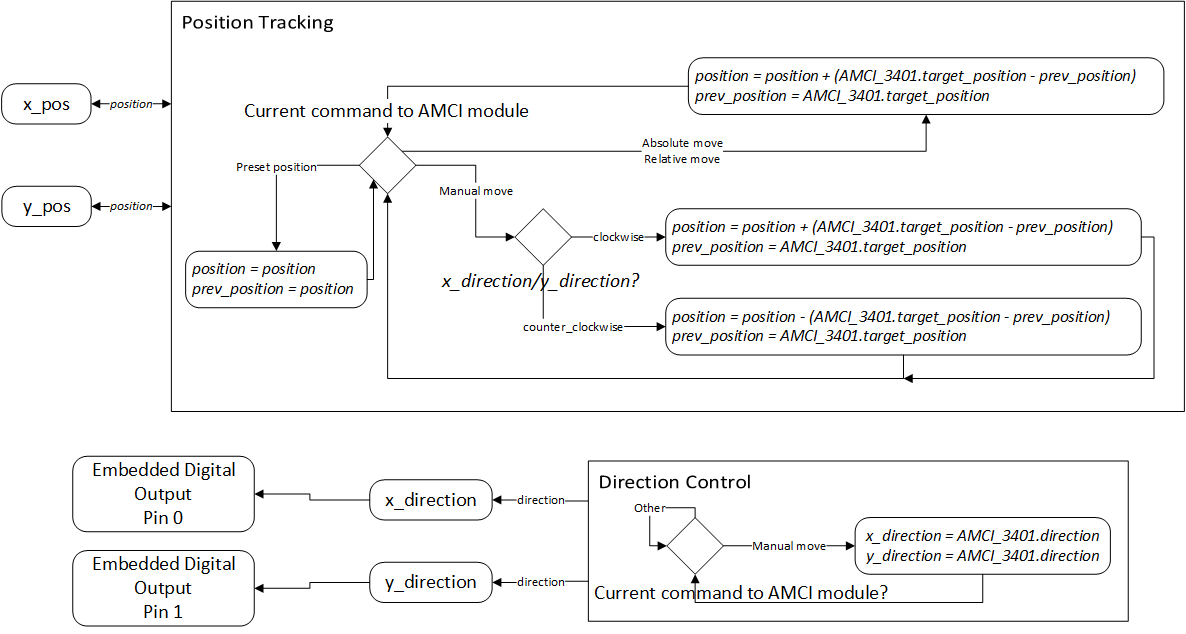
\includegraphics[width=\textwidth]{figures/cncMachine/position_direction}
		\caption{The two routines for managing direction and position}
		\label{fig:Direction and Positional Tracking}
	\end{figure}
	
				\begin{description}
					\item[Absolute Move, Relative Move] \hfill \\
						Relative Moves are treated by the rest of the code as usual. Absolute Moves must be preceded by a Preset Current Position command with the position set to x\_pos and y\_pos. A function monitors the directional state of the AMCI 3401 modules and mirrors this onto the direction output pins. The same function measures the change in position since last scan and adds this to x\_pos and y\_pos.
					\item[Manual Move] \hfill \\
						All manual moves, whether clockwise or anticlockwise, are sent to the AMCI 3401 modules as Manual Move Clockwise at the correct speed. The x\_direction and y\_direction bits need to be explicitly set with each Manual Move command to operate in the required direction. Since the AMCI 3401 module thinks it is always moving clockwise (even when it's not), it's internal position state is no longer correct. Another function measures the change in position since last scan and depending on the direction of movement, adds or subtracts this value to x\_pos and y\_pos.
					\item[Preset Current Position] \hfill \\
						Change the value of x\_pos and y\_pos to mirror the position state in the AMCI 3401 controller.
				\end{description}
				
				
	\section{checkLimitSwitch}
	\label{sec:PLC-flowcharts-limit}
		The checkLimitSwitch program is run in a Periodic Task of 10ms and monitors the four limit switches. Upon detecting a rising edge from one of these limit switches, it sets the appropriate boundaryFault value (boundaryFaultX for the X limit switches and boundaryFaultY for the Y limit switches).
		
		If the boundaryFaultDisable is NOT set, it will assume that unintended operation has occurred and an immediate stop command to the stepper motor modules halting all operation. If boundaryFaultDisable IS set then this operation does not happen (used in a situation where motorControl or the Governor are expecting a limit switch input. Eg, boundary checking or waiting for user to manually toggle the switch).

\chapter{PLC State Machine Flowcharts}
\label{ch:PLC-flowcharts}


\section{Communications State Machine}
\label{sec:PLC-flowcharts-comms}

	\begin{center}
		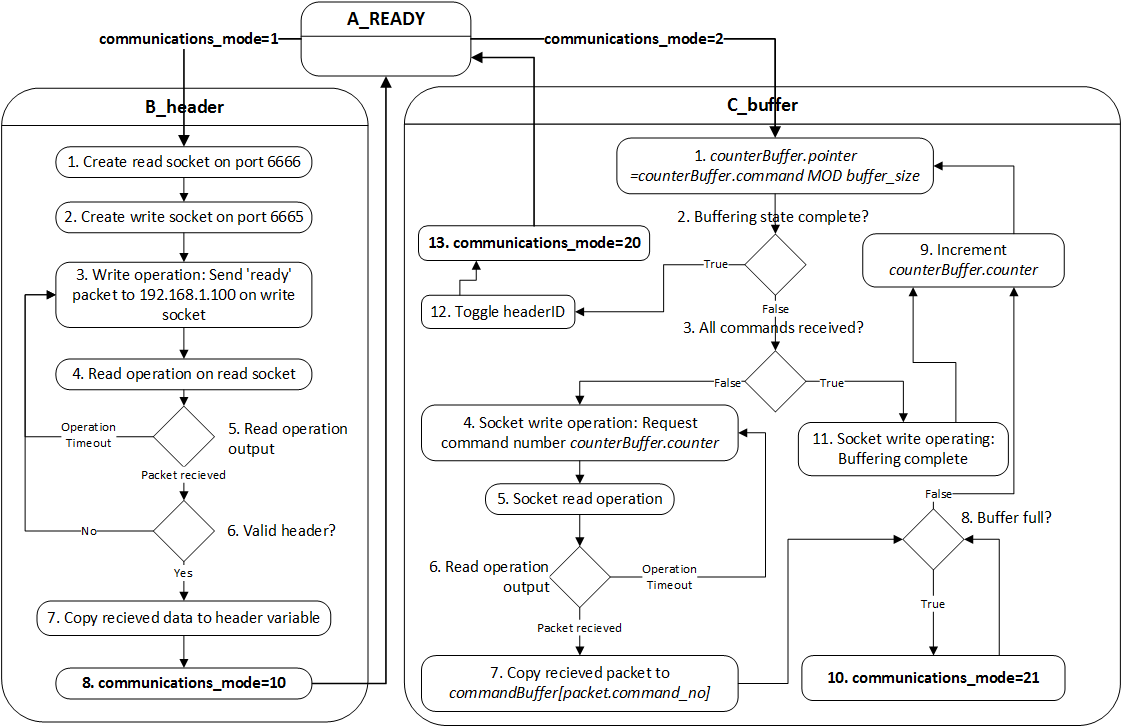
\includegraphics[width=\textwidth]{figures/cncMachine/communications}
		\captionof{figure}{Communications program: States and State Actions}
		\label{fig:communicationsStates}
	\end{center}

\section{motorControl State Machine}
\label{sec:PLC-flowcharts-motor}
	\begin{center}
		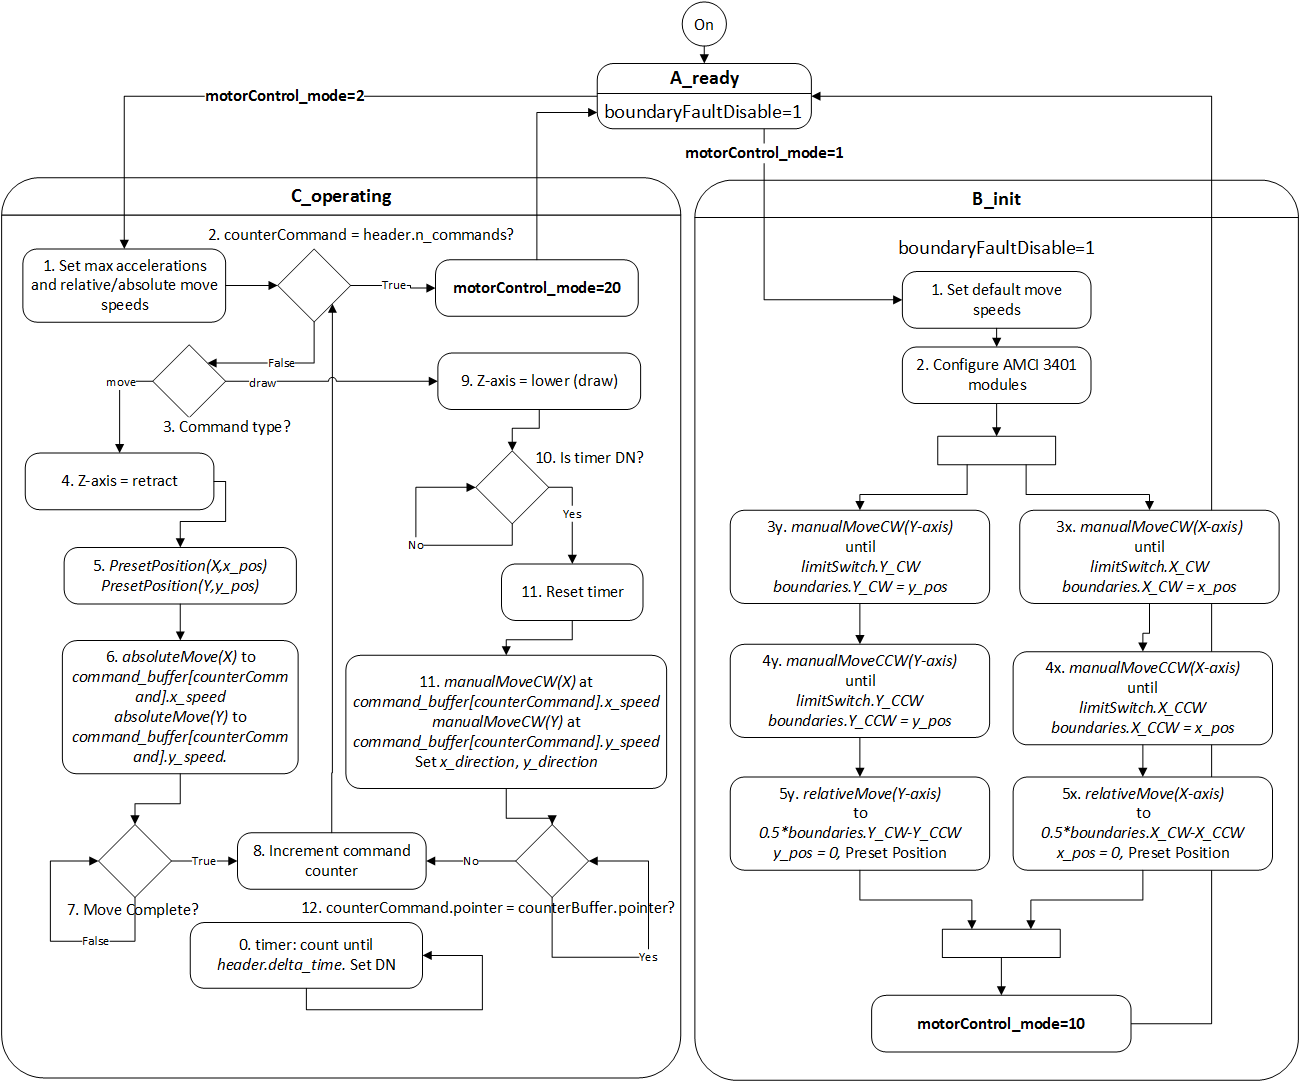
\includegraphics[width=\textwidth]{figures/cncMachine/motorControl}
		\captionof{figure}{motorControl Program: States and State Actions}
		\label{fig:motorControlStates}
	\end{center}

	\subsubsection{Introduction to the AMCI 3401 Stepper Module}
			The main purpose of the motorControl program is to communicate with the two AMCI 3401 Stepper Motor Modules. Their primary role is to send two types of control signals to the stepper motor modules:\\
			\begin{description}
				\item[Step Output] \hfill \\
					A $5V$ square pulse output, with each rising edge signifying a single step of the motor.
				\item[Direction Output] \hfill \\
					A $5V$ boolean output that defines which direction the stepper motors should turn.
			\end{description}
			The modules takes its input by asynchronously monitoring a 16-byte command word on the PLC and mirror it internally. All commands given by the motorControl program involving modifying this command word. \\
			In addition, the module monitors its relative position and operating state by providing a 16-byte status word.\\
			The modules feature a broad range of commands, but the those used by the DoodleBot system are:
			\begin{description}
				\item[Absolute Move] \hfill \\
					Given a position in space (relative to the preset origin position), the AMCI module creates the appropriate velocity profile to get there (within the acceleration/deceleration/top speed parameter limits).
				\item[Relative Move] \hfill \\
					Given a distance to travel (from the current position), the AMCI module creates the appropriate velocity profile to get there (within the acceleration/deceleration/top speed parameter limits).
				\item[Manual Move] \hfill \\
					Manual type moves are actually classified as two separate commands defining the direction of the move  - manual move clockwise, and manual move counterclockwise. These moves accelerate to the programmed speed at the acceleration rate and travel until stopped. While moving in this state, the programmed speed can be changed without having to stop and restart.
				\item[Immediate Stop] \hfill \\
					An immediate stop command stops all current motion.
				\item[Preset Current Position] \hfill \\
					Sets the internal position memory of the module to a position defined in the command word.
			\end{description}

\subsection{Position and Direction Control}
\label{sec:PLC-flowcharts-pos}

	\begin{figure}[htbp!]
		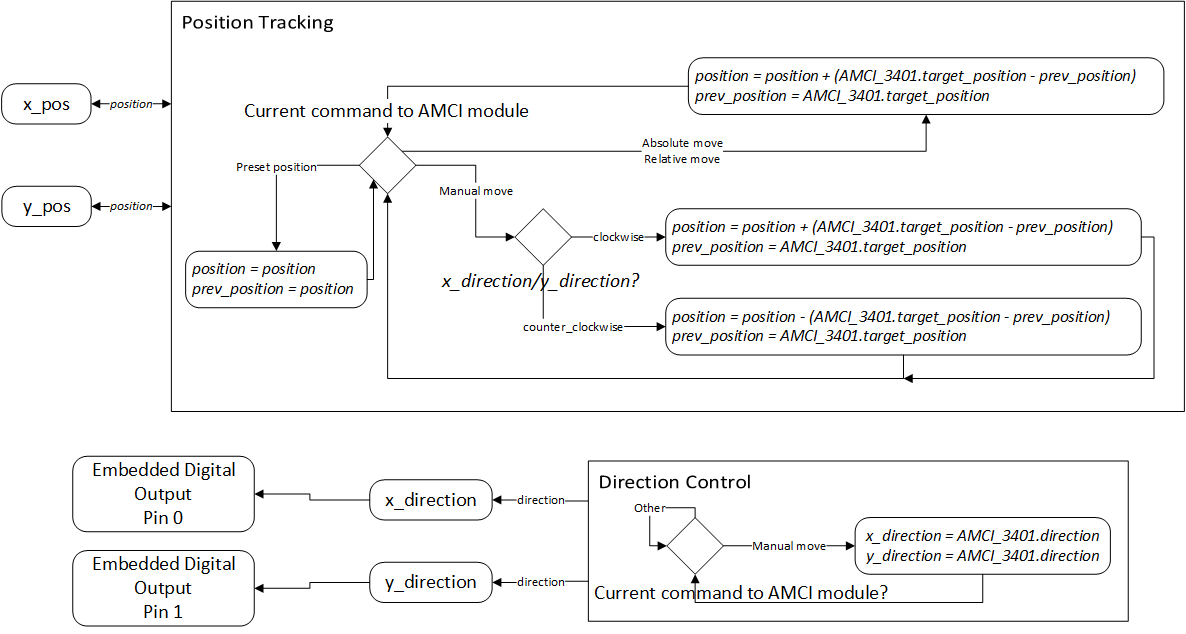
\includegraphics[width=\textwidth]{figures/cncMachine/position_direction}
		\caption{The two routines for managing direction and position}
		\label{fig:Direction and Positional Tracking}
	\end{figure}
	
				\begin{description}
					\item[Absolute Move, Relative Move] \hfill \\
						Relative Moves are treated by the rest of the code as usual. Absolute Moves must be preceded by a Preset Current Position command with the position set to x\_pos and y\_pos. <blah> function monitors the directional state of the AMCI 3401 modules and mirrors this onto the direction output pins. <gah> function measures the change in position since last scan and adds this to x\_pos and y\_pos.
					\item[Manual Move] \hfill \\
						All manual moves, whether clockwise or anticlockwise, are sent to the AMCI 3401 modules as Manual Move Clockwise at the correct speed. The x\_direction and y\_direction bits need to be explicitly set with each Manual Move command to operate in the required direction. Since the AMCI 3401 module thinks it is always moving clockwise (even when it's not), it's internal position state is no longer correct. Function <gah> measures the change in position since last scan and depending on the direction of movement, adds or subtracts this value to x\_pos and y\_pos.
					\item[Preset Current Position] \hfill \\
						Change the value of x\_pos and y\_pos to mirror the position state in the AMCI 3401 controller.
				\end{description}
\end{appendices}


\singlespacing

% the back matter
\clearpage
\bibliography{references}
\addcontentsline{toc}{chapter}{References}
\bibliographystyle{plainnat}
%\chapter*{Colophon}

\begin{center}
\parbox{200pt}{\raggedright\lettrine[lines=3,slope=-2pt,nindent=-4pt]{\textcolor{Crimson}{T}}{his thesis was typeset} using \LaTeX, originally developed by Leslie Lamport and based on Donald Knuth's \TeX. The body text is set in 11 point Arno Pro, designed by Robert Slimbach in the style of book types from the Aldine Press in Venice, and issued by Adobe in 2007. A template, which can be used to format a PhD thesis with this look and feel, has been released under the permissive \textsc{mit} (\textsc{x}11) license, and can be found online at \href{https://github.com/suchow/}{github.com/suchow/} or from the author at \href{mailto:suchow@fas.harvard.edu}{suchow@post.harvard.edu}.
}
\end{center}

\end{document}
